\documentclass[13pt,a4paper]{report}
\usepackage[utf8x]{inputenc}
% \usepackage[vietnamese=nohyphenation]{hyphsubst}
\usepackage[vietnamese, main=english]{babel}
\usepackage{titlesec, blindtext, color}
\usepackage[table,xcdraw]{xcolor}
\usepackage{booktabs}
\usepackage{multicol}
\usepackage{multirow}
\usepackage{titlesec}
\usepackage{amsmath}
\usepackage{amssymb}
\usepackage{adjustbox}
\usepackage{array}
\usepackage{pbox}
\usepackage{caption}
\usepackage{float}
\usepackage{cite}


% Unnumbered chapter heading "Chương N. ..." that still sets chapter N, so that \label after it,
% section/figure/table/equation numbers and \ref all use N
\newcommand{\mychapter}[2]{
    \chapter*{#2}
    \setcounter{chapter}{\numexpr#1-1\relax}
    \refstepcounter{chapter}
    \addcontentsline{toc}{chapter}{#2}
    }
% \setcounter{tocdepth}{4}


\definecolor{gray75}{gray}{0.75}
\newcommand{\hsp}{\hspace{15pt}}
\titleformat{\chapter}[hang]{\small\bfseries}{\thechapter\hsp\textcolor{gray75}{|}\hsp}{0pt}{\Huge\bfseries}
\usepackage[left=3cm,right=2cm,top=2.5cm,bottom=3cm]{geometry}
\setlength{\parindent}{1cm}
\usepackage{indentfirst}
\setlength{\parskip}{6pt}
\usepackage{sectsty}
\chapterfont{\centering}
\renewcommand{\baselinestretch}{1.3} %format distance between lines
\usepackage{xcolor}
\usepackage[utf8]{vietnam}
\usepackage[unicode]{hyperref}
\hypersetup{
colorlinks = false,
linkbordercolor = {white}
}
\usepackage{graphicx}
\usepackage{lmodern}
\usepackage[font=small,labelfont=bf]{caption} % Required for specifying captions to tables and figures
\usepackage{bm}
\usepackage[para]{footmisc}
\usepackage{amsfonts}
\usepackage{afterpage}
\usepackage{tikz}
\usepackage{pdfpages}
\usepackage{xspace}
\usepackage{listings}
\usepackage{animate}

\usetikzlibrary{calc,arrows.meta,positioning,decorations.pathreplacing}
\usepackage{frontespizio}
% \usepackage[perpage]{footmisc}
\usepackage{perpage}
\MakePerPage{footnote}
\usepackage{longtable}
\usepackage{ragged2e}
\usepackage{scrextend}
\usepackage{algorithm}
\usepackage{algpseudocode}
% format titile chapter section ...
\titleformat{\chapter}[display]
{\large}
{
	\large\MakeUppercase{\chaptertitlename}~\thechapter}
{1pc}
{\titlerule\huge}

\titleformat*{\section}{\normalfont \Large}
\titleformat*{\subsection}{\normalfont \large}

\lstset{frame=tb,
  language=python,
  aboveskip=3mm,
  belowskip=3mm,
  showstringspaces=false,
  columns=flexible,
  basicstyle={\small\ttfamily},
  numbers=none,
  numberstyle=\tiny\color{gray},
  keywordstyle=\color{blue},
  breaklines=true,
  breakatwhitespace=true,
  tabsize=3
}

\hypersetup{
    urlcolor=cyan
}

% Vietnamese names for captions and generated lists
\addto\captionsenglish{%
  \renewcommand{\figurename}{Hình}%
  \renewcommand{\tablename}{Bảng}%
  \renewcommand{\contentsname}{Mục lục}%
  \renewcommand{\bibname}{Tài liệu tham khảo}%
  \renewcommand{\listfigurename}{Danh sách hình vẽ}%
  \renewcommand{\listtablename}{Danh sách bảng biểu}%
}
\floatname{algorithm}{Thuật toán}
\algrenewcommand\algorithmicrequire{\textbf{Đầu vào:}}
\algrenewcommand\algorithmicensure{\textbf{Đầu ra:}}

% Diagram styles (shared with the slides)
\tikzset{
  box/.style={draw, rounded corners=2pt, align=center, inner sep=3pt, font=\small},
  cbox/.style={box, draw=blue!60!black, fill=blue!8},
  pbox/.style={box, draw=orange!80!black, fill=orange!12},
  gbox/.style={box, draw=green!50!black, fill=green!10},
  itemnode/.style={circle, draw=blue!60!black, fill=blue!10, minimum size=6.5mm, inner sep=0pt, font=\small},
  elemnode/.style={rectangle, draw=orange!80!black, fill=orange!15, minimum size=6mm, inner sep=0pt, font=\small},
  chosen/.style={fill=green!25, draw=green!50!black, very thick},
  arr/.style={-{Stealth[length=2.2mm]}, thick},
}

% Thesis information: edit here
\newcommand{\todo}[1]{\textcolor{red}{#1}}
\newcommand{\tacgia}{Trương Thế Dũng}
\newcommand{\tacgiaHoa}{TRƯƠNG THẾ DŨNG}
\newcommand{\tendetai}{TÌM KIẾM CỤC BỘ ĐƯỢC HƯỚNG DẪN BỞI MẠNG NƠ-RON ĐỒ THỊ CHO BÀI TOÁN CÁI TÚI HỢP TẬP}
\newcommand{\tendetaiEn}{Graph Neural Network-Guided Local Search for the Set-Union Knapsack Problem}
\newcommand{\nganh}{\todo{[Tên ngành]}}
\newcommand{\nganhHoa}{\todo{[TÊN NGÀNH]}}
\newcommand{\chuyennganh}{\todo{[Tên chuyên ngành]}}
\newcommand{\maso}{\todo{[Mã số]}}
\newcommand{\gvhd}{\todo{[Học hàm, học vị, họ và tên cán bộ hướng dẫn]}}
\newcommand{\namhoc}{2026}

% Short names used in the text
\newcommand{\addstar}{ADD$^{*}$\xspace}

\begin{document}
%\maketitle

\begin{titlepage}
    %doubleshot titlepage's border
    \begin{tikzpicture}[overlay,remember picture]
        \draw [line width=0.8mm]
            ($ (current page.north west) + (2.9cm,-2.4cm) $)
            rectangle
            ($ (current page.south east) + (-1.9cm,2.9cm) $);
        \draw [line width=0.2mm]
            ($ (current page.north west) + (3cm,-2.5cm) $)
            rectangle
            ($ (current page.south east) + (-2cm,3cm) $);
    \end{tikzpicture}

	\begin{center}
		{\fontsize{12}{1.3}\selectfont \textbf{ĐẠI HỌC QUỐC GIA HÀ NỘI\\TRƯỜNG ĐẠI HỌC CÔNG NGHỆ}}

		\vspace{1.25cm}

		
\includegraphics[clip, scale=1]{Logo_UET.jpg}

		\vspace{1.25cm}

		{\fontsize{14}{1.5}\selectfont \textbf{\tacgiaHoa}}

		\vspace{1.5cm}

		{\fontsize{18}{24}\selectfont \textbf{\tendetai}}
	\end{center}

        \vspace{2cm}

        \begin{center}
            {\fontsize{14}{1.5}\selectfont \textbf{LUẬN VĂN THẠC SĨ \nganhHoa}}
        \end{center}

	\vfill
	\begin{center}
		{\fontsize{12}{1.3}\selectfont \textbf{HÀ NỘI -- \namhoc}}
	\end{center}

\end{titlepage}

\begin{titlepage}
    %doubleshot titlepage's border
    \begin{tikzpicture}[overlay,remember picture]
        \draw [line width=0.8mm]
            ($ (current page.north west) + (2.9cm,-2.4cm) $)
            rectangle
            ($ (current page.south east) + (-1.9cm,2.9cm) $);
        \draw [line width=0.2mm]
            ($ (current page.north west) + (3cm,-2.5cm) $)
            rectangle
            ($ (current page.south east) + (-2cm,3cm) $);
    \end{tikzpicture}

	\begin{center}
		{\fontsize{12}{1.3}\selectfont \textbf{ĐẠI HỌC QUỐC GIA HÀ NỘI\\TRƯỜNG ĐẠI HỌC CÔNG NGHỆ}}

		\vspace{2cm}

		{\fontsize{14}{1.5}\selectfont \textbf{\tacgiaHoa}}

		\vspace{1.5cm}

		{\fontsize{18}{24}\selectfont \textbf{\tendetai}}
	\end{center}

        \vspace{1.5cm}

        {\fontsize{13}{20}\selectfont
        \hspace*{2.5cm}Ngành: \nganh\\
        \hspace*{2.5cm}Chuyên ngành: \chuyennganh\\
        \hspace*{2.5cm}Mã số: \maso
        }

        \vspace{1.5cm}

        \begin{center}
            {\fontsize{14}{1.5}\selectfont \textbf{LUẬN VĂN THẠC SĨ \nganhHoa}}
        \end{center}

        \vspace{1cm}

        {\fontsize{13}{20}\selectfont
        \hspace*{2.5cm}\textbf{CÁN BỘ HƯỚNG DẪN KHOA HỌC:}\\
        \hspace*{2.5cm}\gvhd
        }

	\vfill
	\begin{center}
		{\fontsize{12}{1.3}\selectfont \textbf{HÀ NỘI -- \namhoc}}
	\end{center}

\end{titlepage}

\fontsize{12}{12}\selectfont

\pagenumbering{gobble}
\section*{\centering LỜI CAM ĐOAN}

Tôi xin cam đoan luận văn ``\textit{Tìm kiếm cục bộ được hướng dẫn bởi mạng nơ-ron đồ thị cho bài toán cái túi hợp tập}'' là công trình nghiên cứu của riêng tôi, được thực hiện dưới sự hướng dẫn khoa học của \gvhd. Các kết quả thực nghiệm trình bày trong luận văn do tôi trực tiếp cài đặt, chạy và ghi nhận; mã nguồn và dữ liệu kết quả được lưu trữ cùng luận văn. Các số liệu của những công trình khác được trích dẫn đầy đủ từ các tài liệu đã công bố.

Tôi xin chịu hoàn toàn trách nhiệm về tính trung thực của các nội dung trong luận văn này.

\vspace{1cm}
\begin{flushright}
\begin{minipage}{7cm}
\centering
Hà Nội, ngày \todo{...} tháng \todo{...} năm \namhoc\\
\textbf{Học viên}\\[2.5cm]
\textbf{\tacgia}
\end{minipage}
\end{flushright}

\newpage

\section*{\centering LỜI CẢM ƠN}

Tôi xin bày tỏ lòng biết ơn sâu sắc tới \gvhd, người đã tận tình hướng dẫn, định hướng và góp ý cho tôi trong suốt quá trình thực hiện luận văn. Những trao đổi về tìm kiếm cục bộ và tối ưu tổ hợp đã giúp tôi nhìn bài toán theo góc độ của người làm tối ưu, từ đó đặt phần học máy vào đúng chỗ trong một thuật toán tìm kiếm.

Tôi xin cảm ơn các thầy cô giáo Trường Đại học Công nghệ, Đại học Quốc gia Hà Nội đã truyền đạt kiến thức và tạo điều kiện thuận lợi cho tôi trong quá trình học tập và nghiên cứu.

Cuối cùng, tôi xin cảm ơn gia đình và bạn bè đã luôn động viên, ủng hộ tôi trong suốt thời gian qua.

\newpage

\section*{\centering TÓM TẮT}

\textbf{Tóm tắt:} Bài toán cái túi hợp tập (SUKP) là một biến thể NP-khó của bài toán cái túi, trong đó mỗi item là một tập element có trọng số và trọng số của element dùng chung chỉ được tính một lần. Các thuật toán tìm kiếm cục bộ tốt nhất cho SUKP, như E2LS, dựa vào một luật viết tay là tỉ số giá trị trên trọng số để quyết định thêm item nào. Luận văn này giữ nguyên khung E2LS và chỉ thay đúng một thành phần, bước xếp hạng ứng viên của toán tử ADD*, bằng một hàm được học. Luận văn cài đặt lại E2LS bằng C++ với giao diện Python cho phép thay hàm xếp hạng, thiết kế một mạng nơ-ron đồ thị trên đồ thị hai phía item--element với số tham số không phụ thuộc kích thước instance, và huấn luyện hàm xếp hạng theo hai cách: học tăng cường bằng DQN trên từng instance, và học bắt chước từ nhãn tối ưu được tính bằng tìm kiếm vét cạn trên các instance sinh ngẫu nhiên. Bộ xếp hạng học bắt chước được tham số hóa như một hiệu chỉnh của luật tỉ số, nên khi chưa huấn luyện nó trùng với thuật toán gốc. Trên các instance kiểm định chưa gặp, bộ xếp hạng nâng tỉ lệ chọn đúng ứng viên tối ưu từ 60.9\% lên 71.3\% và giảm regret từ 0.71\% xuống 0.44\%. Với một lần chạy 30 giây, bản cài đặt E2LS đạt lời giải tốt nhất đã biết trên 17/30 instance của Set I và có khoảng cách trung bình 1.45\% trên Set II. Luận văn cũng phân tích chi phí suy luận của việc xếp hạng bằng mạng tại mỗi nút tìm kiếm và đề xuất quy trình đánh giá cùng số bước và cùng thời gian cho các hàm xếp hạng học được.

\textbf{Từ khóa:} bài toán cái túi hợp tập, tìm kiếm cục bộ, học tăng cường, mạng nơ-ron đồ thị, học máy cho tối ưu tổ hợp.

\vspace{0.8cm}

\section*{\centering ABSTRACT}

\textbf{Abstract:} The Set-Union Knapsack Problem (SUKP) is an NP-hard variant of the knapsack problem in which each item is a set of weighted elements and a shared element is paid only once. The best local search algorithms for SUKP, such as E2LS, rely on a hand-written value-weight ratio to decide which item to add. This thesis keeps the E2LS framework unchanged and replaces exactly one component, the candidate ranking inside the ADD* operator, with a learned function. We reimplement E2LS in C++ with a Python interface that accepts any ranking function, design a graph neural network over the item--element bipartite graph whose parameter count does not depend on the instance size, and train the ranking function in two ways: per-instance deep Q-learning, and imitation of optimal labels computed by exhaustive search on randomly generated instances. The imitation ranker is parameterised as a correction to the ratio rule, so an untrained model reproduces the original algorithm. On unseen validation instances, the learned ranker raises the rate of picking an optimal candidate from 60.9\% to 71.3\% and lowers the regret from 0.71\% to 0.44\%. With a single 30-second run, the reimplemented E2LS matches the best-known solution on 17 of the 30 Set I instances and is within 1.45\% of it on average on Set II. We also analyse the inference cost of ranking with the network at every search node, and propose an equal-steps and equal-time protocol for evaluating learned rankers on the benchmark.

\textbf{Keywords:} set-union knapsack problem, local search, reinforcement learning, graph neural network, machine learning for combinatorial optimization.

\newpage

\begin{titlepage}
    \pagenumbering{gobble}
    \tableofcontents
\end{titlepage}

\section*{\centering DANH MỤC KÝ HIỆU VÀ CHỮ VIẾT TẮT}

\begin{center}
\renewcommand{\arraystretch}{1.15}
\begin{tabular}{p{2.6cm}p{11.8cm}}
\toprule
\textbf{Ký hiệu} & \textbf{Ý nghĩa} \\
\midrule
SUKP & Bài toán cái túi hợp tập (Set-Union Knapsack Problem) \\
BMCP & Bài toán phủ cực đại có ngân sách (Budgeted Maximum Coverage Problem) \\
E2LS & Thuật toán tìm kiếm cục bộ hiệu quả của Zhu và Luo (Efficient and Effective Local Search) \\
\addstar & Toán tử thêm lại nhiều phần tử theo cây rẽ nhánh trong E2LS \\
RL & Học tăng cường (Reinforcement Learning) \\
MDP & Quá trình quyết định Markov (Markov Decision Process) \\
DQN & Mạng Q sâu (Deep Q-Network) \\
GNN & Mạng nơ-ron đồ thị (Graph Neural Network) \\
GA & Giải thuật di truyền (Genetic Algorithm) \\
BKS & Lời giải tốt nhất đã biết (Best-Known Solution) \\
$m$, $n$ & Số item và số element của một instance \\
$p_i$, $w_j$, $C$ & Lợi nhuận của item $i$, trọng số của element $j$, sức chứa của túi \\
$U_i$ & Tập element mà item $i$ phủ \\
$P(S)$, $W(S)$ & Tổng lợi nhuận và tổng trọng số (hợp tập) của lời giải $S$ \\
$AW(S,i)$ & Trọng số tăng thêm khi thêm $i$ vào $S$ (hoặc giải phóng khi bỏ $i$ khỏi $S$) \\
$R(S,i)$ & Tỉ số giá trị trên trọng số $p_i/AW(S,i)$ \\
$FC$ & Tập ứng viên khả thi tại một nút \addstar \\
$r_{num}$, $a_{num}$ & Số item được thử bỏ và số ứng viên được rẽ nhánh tại mỗi nút \addstar \\
$Q_\theta(s,a)$ & Hàm giá trị hành động được xấp xỉ bởi mạng nơ-ron tham số $\theta$ \\
$\gamma$ & Hệ số chiết khấu \\
\bottomrule
\end{tabular}
\end{center}

\newpage

\begin{titlepage}
    \pagenumbering{gobble}
    \listoffigures
\end{titlepage}

\begin{titlepage}
    \pagenumbering{gobble}
    \listoftables
\end{titlepage}

\pagenumbering{arabic}
\setcounter{page}{1}
\mychapter{1}{Chương 1. Tổng quan}\label{ch:chap1}

\section{Đặt vấn đề}

Bài toán cái túi (knapsack) là một trong những mô hình kinh điển nhất của tối ưu tổ hợp: chọn một tập con các vật có giá trị sao cho tổng giá trị lớn nhất mà tổng trọng lượng không vượt quá sức chứa của túi~\cite{Kellerer2004}. Trong nhiều ứng dụng thực tế, chi phí của một lựa chọn không phải là tổng chi phí của từng vật một cách độc lập, vì các vật có thể \emph{dùng chung tài nguyên}. Khi đó tài nguyên dùng chung chỉ phải trả một lần. Bài toán cái túi hợp tập (Set-Union Knapsack Problem, SUKP) do Goldschmidt, Nehme và Yu đề xuất năm 1994~\cite{Goldschmidt1994} mô hình hóa đúng tình huống này: mỗi \emph{item} có một lợi nhuận và là một tập các \emph{element} có trọng số; trọng lượng của một lựa chọn là tổng trọng số của \emph{hợp} các element mà các item được chọn phủ lên.

SUKP xuất hiện trong nhiều lĩnh vực như sản xuất linh hoạt~\cite{Goldschmidt1994}, ra quyết định tài chính~\cite{Khuller1999,Kellerer2004}, nén dữ liệu, tối ưu mạng định nghĩa bằng phần mềm và lựa chọn dự án đầu tư~\cite{Wei2019,Zhu2022}. Bài toán là NP-khó: khi không có hai item nào dùng chung element, SUKP trở thành bài toán cái túi 0-1~\cite{Goldschmidt1994,Arulselvan2014}. Vì vậy, với các instance có hàng trăm đến hàng nghìn item, các phương pháp chính xác khó áp dụng, và các thuật toán metaheuristic, đặc biệt là tìm kiếm cục bộ dựa trên tabu~\cite{Wei2019,Wei2021,Zhu2022}, đang cho kết quả tốt nhất.

Các thuật toán tìm kiếm cục bộ tốt nhất hiện nay đều dựa vào những \emph{luật đánh giá viết tay}. Thuật toán E2LS~\cite{Zhu2022}, một trong những phương pháp mạnh nhất cho SUKP, quyết định thêm item nào vào lời giải dựa trên tỉ số giữa lợi nhuận của item và phần trọng số mà item đó làm tăng thêm. Tỉ số này đơn giản, rẻ và hiệu quả, nhưng về bản chất là một đánh giá \emph{tham lam một bước}: nó đo lợi ích tức thời của một nước đi mà không biết nước đi đó mở ra hay đóng lại những khả năng nào ở các bước sau, chẳng hạn khi hai item dùng chung nhiều element nên chọn cùng nhau thì tốt hơn chọn riêng lẻ.

Song song với đó, học máy cho tối ưu tổ hợp đã phát triển mạnh trong khoảng mười năm gần đây~\cite{Bengio2021}. Một hướng đặc biệt hiệu quả là \emph{không thay thế thuật toán tối ưu, mà chỉ học một thành phần của nó}: học quy tắc rẽ nhánh trong branch-and-bound~\cite{Gasse2019}, hay học hàm heuristic trong giải thuật đàn kiến~\cite{Ye2023DeepACO}. Cách tiếp cận này giữ nguyên các đảm bảo và cơ chế tìm kiếm đã được kiểm chứng của thuật toán gốc, đồng thời cho phép mô hình học được những quy luật mà luật viết tay bỏ sót.

Luận văn này theo hướng tiếp cận trên cho SUKP. Câu hỏi nghiên cứu đặt ra là: \emph{có thể học một hàm đánh giá nước đi tốt hơn tỉ số giá trị trên trọng số, và thay nó vào đúng một vị trí trong E2LS, để cải thiện chất lượng tìm kiếm hay không?}

\section{Bài toán cái túi hợp tập}

Hình~\ref{fig:sukp_example} minh họa một instance nhỏ. Có ba item với lợi nhuận $p_1=6$, $p_2=5$, $p_3=4$ và bốn element với trọng số lần lượt là $3,2,4,3$; sức chứa $C=9$. Item 1 phủ $\{e_1,e_2\}$, item 2 phủ $\{e_2,e_3\}$, item 3 phủ $\{e_3,e_4\}$. Nếu tính chi phí theo từng item như bài toán cái túi thông thường, chọn item 1 và 2 tốn $5+6=11>C$. Nhưng trong SUKP, element $e_2$ được hai item dùng chung chỉ tính một lần, nên lời giải $S=\{1,2\}$ có trọng lượng $W(S)=3+2+4=9\le C$ và lợi nhuận $P(S)=11$, là lời giải tối ưu.

\begin{figure}[H]
\centering
\begin{tikzpicture}[x=1.5cm,y=1.2cm]
  \node[itemnode,chosen] (i1) at (0.67,2.2) {$1$};
  \node[itemnode,chosen] (i2) at (2.00,2.2) {$2$};
  \node[itemnode]        (i3) at (3.33,2.2) {$3$};
  \node[above=0.5mm of i1, font=\scriptsize] {$p_1=6$};
  \node[above=0.5mm of i2, font=\scriptsize] {$p_2=5$};
  \node[above=0.5mm of i3, font=\scriptsize] {$p_3=4$};
  \node[elemnode,chosen] (e1) at (0.00,0) {$e_1$};
  \node[elemnode,chosen] (e2) at (1.33,0) {$e_2$};
  \node[elemnode,chosen] (e3) at (2.67,0) {$e_3$};
  \node[elemnode]        (e4) at (4.00,0) {$e_4$};
  \node[below=0.5mm of e1, font=\scriptsize] {$w=3$};
  \node[below=0.5mm of e2, font=\scriptsize] {$w=2$};
  \node[below=0.5mm of e3, font=\scriptsize] {$w=4$};
  \node[below=0.5mm of e4, font=\scriptsize] {$w=3$};
  \foreach \i/\j in {1/1,1/2,2/2,2/3} \draw[green!50!black, very thick] (i\i) -- (e\j);
  \foreach \i/\j in {3/3,3/4} \draw[gray!70, thick] (i\i) -- (e\j);
  \node[font=\small, align=left, anchor=west] at (4.6,1.1) {$C=9$\\ $S=\{1,2\}$: $W(S)=9$, $P(S)=11$};
\end{tikzpicture}
\caption{Một instance SUKP nhỏ dưới dạng đồ thị hai phía item--element. Item được chọn và các element chúng phủ được tô màu xanh; element $e_2$ dùng chung nên chỉ tính trọng số một lần.}
\label{fig:sukp_example}
\end{figure}

Biểu diễn đồ thị hai phía trong Hình~\ref{fig:sukp_example} không chỉ để minh họa. Nó cũng là cấu trúc dữ liệu đầu vào của các mạng nơ-ron đồ thị được dùng trong luận văn (Chương~\ref{ch:chap3}): giá trị của việc thêm một item phụ thuộc vào việc các element của nó đã được phủ hay chưa, và được những item nào khác dùng chung.

\section{Mục tiêu và phạm vi nghiên cứu}

Mục tiêu tổng quát của luận văn là xây dựng một bộ giải SUKP kết hợp tìm kiếm cục bộ với học máy, trong đó học máy chỉ đảm nhận một vai trò được xác định rõ, để mọi khác biệt về kết quả có thể quy cho thành phần được học. Cụ thể, luận văn đặt ra các mục tiêu sau:
\begin{enumerate}
  \item Cài đặt lại thuật toán E2LS~\cite{Zhu2022} bằng C++ một cách hiệu quả, có giao diện Python, và kiểm chứng chất lượng trên 60 instance chuẩn của SUKP.
  \item Xác định một điểm cắm (plug-in point) cho học máy trong E2LS: bước xếp hạng các ứng viên tại mỗi nút của toán tử \addstar, nơi bài báo gốc dùng tỉ số giá trị trên trọng số.
  \item Thiết kế một mạng nơ-ron đồ thị trên đồ thị hai phía item--element, có số tham số không phụ thuộc kích thước instance.
  \item Huấn luyện hàm xếp hạng theo hai cách: (i) học tăng cường bằng DQN trên từng instance, và (ii) học bắt chước từ các nhãn tối ưu được sinh bằng tìm kiếm vét cạn trên các instance sinh ngẫu nhiên.
  \item Đánh giá hàm xếp hạng học được so với luật tỉ số gốc về chất lượng xếp hạng và chi phí suy luận, và xây dựng quy trình so sánh hai hàm xếp hạng trên bộ chuẩn ở cùng số bước và cùng thời gian chạy.
\end{enumerate}

Về phạm vi, luận văn chỉ xét SUKP (không xét biến thể BMCP), dùng bộ 60 instance chuẩn gồm Set I~\cite{He2018} và Set II~\cite{Wei2021}, và chỉ thay đổi bước xếp hạng ứng viên của \addstar; các thành phần khác của E2LS (chọn item để bỏ, danh sách tabu, khởi tạo lại) được giữ nguyên. Toàn bộ thực nghiệm chạy trên một máy tính xách tay, không dùng GPU, nên ngân sách thời gian ngắn hơn đáng kể so với các công bố trước (Chương~\ref{ch:chap4}).

\section{Đóng góp của luận văn}

Các đóng góp chính của luận văn gồm:
\begin{itemize}
  \item Một bản cài đặt E2LS bằng C++17 với trạng thái tăng dần (incremental), danh sách tabu bằng băm Zobrist 64 bit, và module Python (\texttt{sukp\_cpp}) cho phép thay hàm xếp hạng ứng viên bằng một hàm Python bất kỳ. Với một lần chạy 30 giây, bản cài đặt đạt lời giải tốt nhất đã biết trên 17/30 instance của Set I và có khoảng cách trung bình 1.45\% trên Set II.
  \item Mô hình hóa việc chọn nước đi của tìm kiếm cục bộ thành một quá trình quyết định Markov, với phần thưởng bằng mức cải thiện lời giải tốt nhất, sao cho mục tiêu học trùng với mục tiêu của tìm kiếm cục bộ.
  \item Một kiến trúc mạng nơ-ron đồ thị cho SUKP với ba loại nút (item, element, nút toàn cục) mà các đặc trưng đầu vào là các đại lượng quen thuộc của bài toán (trọng số tăng thêm, độ phủ của element), được dùng chung cho cả DQN và bộ xếp hạng.
  \item Một bộ xếp hạng học bắt chước được tham số hóa dưới dạng \emph{hiệu chỉnh} của luật tỉ số gốc: khi chưa huấn luyện, nó xếp hạng giống hệt bài báo, và quá trình học chỉ thay đổi những chỗ có lợi. Trên các instance kiểm định, bộ xếp hạng nâng tỉ lệ chọn đúng ứng viên tối ưu từ khoảng 61\% lên khoảng 71\%.
  \item Một phân tích hành vi tìm kiếm và chi phí suy luận, cho thấy khởi tạo lại chiếm tới 21--44\% số bước trên các instance nhỏ và việc gọi mạng tại mỗi nút \addstar làm bước tìm kiếm chậm đi khoảng 6 lần trên instance lớn nhất; từ đó đề xuất các hướng cải tiến cụ thể.
\end{itemize}

\section{Cấu trúc luận văn}

Phần còn lại của luận văn được tổ chức như sau. Chương~\ref{ch:chap2} trình bày cơ sở lý thuyết: định nghĩa hình thức của SUKP, các thuật toán đã có, tìm kiếm cục bộ và tabu, học tăng cường, mạng nơ-ron đồ thị và các hướng học máy cho tối ưu tổ hợp. Chương~\ref{ch:chap3} trình bày phương pháp đề xuất: bộ giải E2LS cài đặt bằng C++, điểm cắm học máy, kiến trúc mạng đồ thị và hai phương án huấn luyện. Chương~\ref{ch:chap4} trình bày thiết lập và kết quả thực nghiệm. Chương~\ref{ch:chap5} tổng kết luận văn và đề xuất các hướng phát triển.

\setcounter{figure}{0}
\setcounter{table}{0}
\mychapter{2}{Chương 2. Cơ sở lý thuyết và các nghiên cứu liên quan}\label{ch:chap2}

Chương này trình bày các kiến thức nền tảng mà luận văn sử dụng. Mục~\ref{sec:sukp_def} định nghĩa bài toán SUKP và bộ dữ liệu chuẩn. Mục~\ref{sec:sukp_algos} tổng quan các thuật toán đã được đề xuất cho SUKP. Mục~\ref{sec:ls} trình bày tìm kiếm cục bộ và tìm kiếm tabu. Mục~\ref{sec:rl} và~\ref{sec:gnn} lần lượt trình bày học tăng cường và mạng nơ-ron đồ thị. Mục~\ref{sec:ml4co} tổng quan các hướng học máy cho tối ưu tổ hợp và xác định vị trí của luận văn.

\section{Bài toán cái túi hợp tập}\label{sec:sukp_def}

\subsection{Định nghĩa hình thức}

Cho một tập $U=\{1,\dots,n\}$ gồm $n$ element, mỗi element $j$ có trọng số $w_j>0$, và một tập $V=\{1,\dots,m\}$ gồm $m$ item, mỗi item $i$ có lợi nhuận $p_i>0$ và tương ứng với một tập con element $U_i\subseteq U$. Quan hệ giữa item và element được cho bởi ma trận $R\in\{0,1\}^{m\times n}$, với $R_{ij}=1$ khi và chỉ khi $j\in U_i$. Cho sức chứa $C>0$. Với một tập item $S\subseteq V$, định nghĩa tổng lợi nhuận và tổng trọng số:
\begin{equation}
P(S)=\sum_{i\in S}p_i,
\qquad
W(S)=\sum_{j\in\bigcup_{i\in S}U_i} w_j .
\label{eq:sukp_pw}
\end{equation}
Bài toán cái túi hợp tập là tìm
\begin{equation}
\max_{S\subseteq V}\ P(S)\quad\text{với ràng buộc}\quad W(S)\le C .
\label{eq:sukp}
\end{equation}
Điểm khác biệt cốt lõi so với bài toán cái túi 0-1 nằm ở $W(S)$: trọng số của một element chỉ được tính \emph{một lần} dù element đó thuộc nhiều item được chọn~\cite{Goldschmidt1994,Wei2021}. Do đó chi phí của một item không cố định mà phụ thuộc vào những item đã có trong lời giải.

\subsection{Mô hình quy hoạch nguyên 0-1}

Đặt biến nhị phân $x_i=1$ nếu item $i$ được chọn và $y_j=1$ nếu element $j$ được phủ. SUKP có thể viết dưới dạng quy hoạch tuyến tính nguyên:
\begin{align}
\max\quad & \sum_{i=1}^{m}p_i x_i \label{eq:ilp_obj}\\
\text{s.t.}\quad & \sum_{j=1}^{n}w_j y_j\le C, \label{eq:ilp_cap}\\
& x_i\le y_j \qquad \forall i\in V,\ \forall j\in U_i, \label{eq:ilp_cover}\\
& x_i,\,y_j\in\{0,1\}. \nonumber
\end{align}
Ràng buộc~\eqref{eq:ilp_cover} buộc mọi element của một item được chọn phải được phủ. Vì mục tiêu không phụ thuộc $y$ và $w_j>0$, ở lời giải tối ưu $y_j=1$ chỉ khi cần thiết, nên~\eqref{eq:ilp_cap} đúng bằng ràng buộc $W(S)\le C$. Mô hình này có $m+n$ biến và $\sum_i|U_i|$ ràng buộc phủ. Wei và Hao cho thấy bộ giải CPLEX dựa trên mô hình 0-1 chỉ chứng minh được tối ưu cho 6 instance nhỏ nhất (85 đến 100 item và element) của bộ chuẩn trong giới hạn hai giờ~\cite{Wei2019}, cho thấy phương pháp chính xác khó mở rộng.

\subsection{Độ phức tạp và các bài toán liên quan}

SUKP là NP-khó: khi các tập $U_i$ đôi một rời nhau, $W(S)=\sum_{i\in S}\sum_{j\in U_i}w_j$ và SUKP trở thành bài toán cái túi 0-1 với trọng lượng item $\sum_{j\in U_i}w_j$~\cite{Goldschmidt1994}. Khi mọi lợi nhuận và trọng số bằng 1, SUKP tương đương bài toán đồ thị con dày đặc nhất trên siêu đồ thị (densest $k$-subhypergraph)~\cite{Arulselvan2014}. SUKP cũng có quan hệ đối ngẫu với bài toán phủ cực đại có ngân sách (BMCP)~\cite{Khuller1999}: BMCP cực đại hóa tổng trọng số element được phủ với ràng buộc tổng chi phí item, tức là đổi vai trò của hàm mục tiêu và ràng buộc~\cite{Zhu2022}. Arulselvan~\cite{Arulselvan2014} chỉ ra rằng thuật toán tham lam của Khuller, Moss và Naor cho BMCP cũng cho một xấp xỉ hằng số với trường hợp đặc biệt của SUKP khi mỗi element thuộc không quá một số hằng tập.

\subsection{Bộ dữ liệu chuẩn}\label{sec:benchmark}

Các nghiên cứu về SUKP thường đánh giá trên hai bộ dữ liệu, tổng cộng 60 instance:
\begin{itemize}
  \item \textbf{Set I} gồm 30 instance với 85 đến 500 item và element, do He và cộng sự đề xuất~\cite{He2018}. Các instance chia làm ba loại theo quan hệ giữa $m$ và $n$: $m>n$, $m=n$ và $m<n$.
  \item \textbf{Set II} gồm 30 instance lớn hơn với 585 đến 1000 item và element, do Wei và Hao đề xuất~\cite{Wei2021}. Lợi nhuận và trọng số được sinh ngẫu nhiên trong đoạn $[1,500]$ theo cách của He và cộng sự.
\end{itemize}
Mỗi instance được đặc trưng bởi bốn tham số và được đặt tên theo dạng \texttt{sukp\_$m$\_$n$\_$\alpha$\_$\beta$}, trong đó $\alpha=\sum_{i,j}R_{ij}/(mn)$ là mật độ của ma trận quan hệ và $\beta=C/\sum_j w_j$ là tỉ lệ sức chứa so với tổng trọng số element~\cite{Zhu2022}. Hai cặp tham số được dùng là $(\alpha,\beta)=(0.10,0.75)$ và $(0.15,0.85)$. Ví dụ \texttt{sukp\_85\_100\_0.10\_0.75} có 85 item, 100 element, mật độ 0.10 và sức chứa bằng 75\% tổng trọng số element.

\section{Các thuật toán giải SUKP}\label{sec:sukp_algos}

\subsection{Thuật toán chính xác và xấp xỉ}

Goldschmidt và cộng sự đề xuất bài toán cùng với một thuật toán quy hoạch động có thời gian chạy hàm mũ~\cite{Goldschmidt1994}. Như đã nêu ở trên, giải mô hình quy hoạch nguyên bằng bộ giải thương mại chỉ khả thi với các instance rất nhỏ~\cite{Wei2019}. Các thuật toán xấp xỉ~\cite{Arulselvan2014} có đảm bảo lý thuyết nhưng chất lượng lời giải trên thực tế thấp hơn nhiều so với các heuristic~\cite{Zhu2022}. Vì vậy hướng nghiên cứu chính cho SUKP là các thuật toán heuristic và metaheuristic.

\subsection{Thuật toán dựa trên quần thể}

He và cộng sự~\cite{He2018} đề xuất thuật toán bầy ong nhân tạo nhị phân (BABC), cùng với bộ dữ liệu Set I. Sau đó nhiều thuật toán bầy đàn và tiến hóa khác được đề xuất. Ozsoydan và Gölcük~\cite{Ozsoydan2023} dùng Q-learning như một hệ thống khuyến nghị chọn giữa các bộ tối ưu PSO, GA và một biến thể lai di truyền--bầy hạt (gbPSO): bộ tối ưu nào đem lại cải thiện sẽ được thưởng và được gọi thường xuyên hơn. Đây là một dạng siêu heuristic (hyper-heuristic~\cite{Burke2013}) dùng học tăng cường ở mức chọn thuật toán, khác với luận văn này, nơi học máy được dùng ở mức chọn nước đi. Gần đây, Zhao và Hifi~\cite{Zhao2024} đề xuất thuật toán tiến hóa thích nghi AES-BM với tập lưu trữ các lời giải ưu tú và đa dạng. Nhìn chung, các phương pháp quần thể phức tạp hơn để thiết kế và kém hơn các phương pháp tìm kiếm cục bộ tốt nhất trên các instance lớn~\cite{Zhu2022}.

\subsection{Thuật toán tìm kiếm cục bộ}

Wei và Hao~\cite{Wei2019} đề xuất I2PLS, thuật toán tìm kiếm cục bộ đầu tiên cho SUKP, xen kẽ một pha tìm kiếm tabu với một pha nhiễu loạn để đến vùng chưa khám phá. KBTS~\cite{Wei2021} dùng một bộ đếm tần suất trong quá trình tìm kiếm tabu để xây dựng một lời giải ``nhân'' (kernel) gồm các item thường xuất hiện trong các lời giải tốt, rồi tìm kiếm tăng cường quanh nhân đó trước khi nhiễu loạn; công trình này cũng đề xuất bộ dữ liệu Set II. Các thuật toán này tìm láng giềng tốt nhất của lời giải hiện tại ở mỗi bước, nhưng láng giềng chứa nhiều nước đi chất lượng thấp, làm giảm hiệu quả~\cite{Zhu2022}.

Zhu và Luo~\cite{Zhu2022} đề xuất E2LS (Efficient and Effective Local Search) cho cả SUKP và BMCP. Ý tưởng chính của E2LS là \emph{thu hẹp vùng tìm kiếm} bằng tỉ số giá trị trên trọng số: chỉ thử bỏ các item có tỉ số thấp nhất, và chỉ rẽ nhánh trên các ứng viên có tỉ số cao nhất khi thêm lại. Toán tử \addstar của E2LS thêm lại nhiều item theo một cây rẽ nhánh có giới hạn, cho phép xét nhiều tổ hợp item mà vẫn nhanh. E2LS dùng danh sách tabu dựa trên lời giải và khởi tạo lại bằng một thủ tục tham lam ngẫu nhiên. Theo báo cáo của tác giả, E2LS đạt hoặc vượt lời giải tốt nhất đã biết trên các bộ dữ liệu chuẩn. E2LS là thuật toán nền của luận văn và được trình bày chi tiết ở Mục~\ref{sec:e2ls}.

Bảng~\ref{tab:sukp_algos} tóm tắt các thuật toán được dùng để so sánh trong Chương~\ref{ch:chap4}.

\begin{table}[H]
\centering
\caption{Các thuật toán cho SUKP được dùng để so sánh.}
\label{tab:sukp_algos}
\small
\begin{tabular}{llll}
\toprule
\textbf{Thuật toán} & \textbf{Loại} & \textbf{Công bố} & \textbf{Bộ dữ liệu báo cáo}\\
\midrule
BABC~\cite{He2018} & Bầy ong nhân tạo nhị phân & 2018 & Set I\\
I2PLS~\cite{Wei2019} & Tìm kiếm cục bộ hai pha lặp & 2019 & Set I\\
KBTS~\cite{Wei2021} & Tìm kiếm tabu dựa trên nhân & 2021 & Set I, Set II\\
E2LS~\cite{Zhu2022} & Tìm kiếm cục bộ với \addstar & 2022 & Set I, Set II\\
QL, gbPSO~\cite{Ozsoydan2023} & Q-learning chọn bộ tối ưu; PSO lai GA & 2023 & Set I\\
AES-BM~\cite{Zhao2024} & Tiến hóa thích nghi & 2024 & Set I\\
\bottomrule
\end{tabular}
\end{table}

\section{Tìm kiếm cục bộ và tìm kiếm tabu}\label{sec:ls}

Tìm kiếm cục bộ bắt đầu từ một lời giải và lặp lại việc di chuyển sang một lời giải \emph{láng giềng}, tức là một lời giải nhận được bằng một thay đổi nhỏ như thêm, bỏ hoặc hoán đổi một phần tử. Một quy tắc chọn nước đi (move evaluation) quyết định láng giềng nào được chọn. Nếu chỉ chấp nhận nước đi cải thiện, thuật toán sẽ dừng ở một cực trị địa phương.

Tìm kiếm tabu~\cite{Glover1989} cho phép đi sang lời giải tệ hơn để thoát khỏi cực trị địa phương, và dùng một bộ nhớ ngắn hạn (danh sách tabu) để cấm quay lại các trạng thái hoặc nước đi gần đây, tránh đi vòng. Có hai dạng chính: tabu theo \emph{thuộc tính} cấm đảo ngược một nước đi trong một số bước, và tabu theo \emph{lời giải} cấm thăm lại chính các lời giải đã thăm. Tabu theo lời giải thường được cài đặt bằng hàm băm: E2LS dùng ba vector băm có độ dài $10^8$, và một lời giải bị cấm nếu cả ba vị trí băm của nó đều đã được đánh dấu~\cite{Zhu2022}. Hai khái niệm quan trọng khác của metaheuristic là \emph{tăng cường} (intensification), tức tập trung tìm quanh các vùng tốt, và \emph{đa dạng hóa} (diversification), tức đưa tìm kiếm đến vùng mới, chẳng hạn bằng khởi tạo lại.

Hiệu quả của tìm kiếm cục bộ phụ thuộc lớn vào quy tắc chọn nước đi. Quy tắc này thường là một heuristic viết tay, như tỉ số giá trị trên trọng số trong E2LS. Luận văn giữ nguyên khung tìm kiếm và chỉ học lại quy tắc này.

\section{Học tăng cường}\label{sec:rl}

\subsection{Quá trình quyết định Markov}

Học tăng cường~\cite{Sutton2018} nghiên cứu cách một tác tử (agent) học chọn hành động thông qua tương tác với môi trường. Bài toán được hình thức hóa bằng quá trình quyết định Markov (MDP) gồm tập trạng thái $\mathcal{S}$, tập hành động $\mathcal{A}(s)$ khả dụng tại trạng thái $s$, hàm chuyển trạng thái và hàm phần thưởng. Tại bước $t$, tác tử ở trạng thái $s_t$, chọn hành động $a_t$ theo chính sách $\pi(a\mid s)$, nhận phần thưởng $r_{t+1}$ và chuyển sang $s_{t+1}$. Mục tiêu là cực đại hóa \emph{return} kỳ vọng
\begin{equation}
G_t=\sum_{k\ge 0}\gamma^k r_{t+k+1},
\end{equation}
với hệ số chiết khấu $\gamma\in[0,1)$. Giá trị $1/(1-\gamma)$ có thể hiểu là tầm nhìn hiệu dụng tính theo số bước.

Hàm giá trị hành động $Q^\pi(s,a)=\mathbb{E}_\pi[G_t\mid s_t=s,a_t=a]$ đo mức tốt của việc chọn $a$ tại $s$ rồi đi theo $\pi$. Hàm giá trị tối ưu $Q^*$ thỏa phương trình Bellman
\begin{equation}
Q^*(s,a)=\mathbb{E}\Big[\,r_{t+1}+\gamma\max_{a'\in\mathcal{A}(s_{t+1})}Q^*(s_{t+1},a')\ \Big|\ s_t=s,\ a_t=a\Big],
\label{eq:bellman}
\end{equation}
và chính sách tối ưu chọn $\arg\max_a Q^*(s,a)$. Đối với người làm tối ưu, $Q^*(s,a)$ chính là \emph{giá trị còn lại} (cost-to-go) của nước đi $a$: tổng cải thiện tốt nhất có thể đạt được nếu đi $a$ rồi tiếp tục tối ưu; phương trình~\eqref{eq:bellman} là đệ quy của quy hoạch động~\cite{Bertsekas1996}.

\subsection{Q-learning}

Khi không gian trạng thái quá lớn để giải~\eqref{eq:bellman} trực tiếp, Q-learning~\cite{Watkins1992} ước lượng $Q^*$ từ các chuyển tiếp mẫu $(s,a,r,s')$:
\begin{equation}
Q(s,a)\leftarrow Q(s,a)+\alpha\Big[\,r+\gamma\max_{a'}Q(s',a')-Q(s,a)\,\Big],
\end{equation}
với bước học $\alpha$. Q-learning dạng bảng hội tụ về $Q^*$ khi mọi cặp trạng thái--hành động được thăm vô hạn lần và bước học giảm dần phù hợp~\cite{Watkins1992}. Để mọi hành động đều được thử, tác tử cần \emph{thăm dò}: chính sách $\varepsilon$-greedy chọn hành động ngẫu nhiên với xác suất $\varepsilon$; chính sách softmax (Boltzmann) chọn $a$ với xác suất tỉ lệ với $\exp(Q(s,a)/\tau)$, với nhiệt độ $\tau$. Thăm dò trong học tăng cường tương ứng với đa dạng hóa trong metaheuristic.

\subsection{Mạng Q sâu}

Với SUKP, mỗi lời giải là một vector nhị phân độ dài $m$, nên có tới $2^m$ trạng thái và không thể lưu $Q$ dưới dạng bảng. Mạng Q sâu (DQN)~\cite{Mnih2015} xấp xỉ $Q$ bằng một mạng nơ-ron $Q_\theta$ và cực tiểu hóa sai số so với đích Bellman:
\begin{equation}
y=r+\gamma\max_{a'}Q_{\bar\theta}(s',a'),
\qquad
\mathcal{L}(\theta)=\mathbb{E}_{(s,a,r,s')\sim\mathcal{D}}\big[(Q_\theta(s,a)-y)^2\big].
\label{eq:dqn}
\end{equation}
Hai kỹ thuật ổn định quá trình học là: (i) \emph{bộ nhớ phát lại} (replay buffer) $\mathcal{D}$ lưu các chuyển tiếp cũ và lấy mẫu ngẫu nhiên, làm giảm tương quan giữa các mẫu liên tiếp; và (ii) \emph{mạng đích} $Q_{\bar\theta}$ là bản sao của $Q_\theta$ được cập nhật định kỳ, tránh việc đích học thay đổi liên tục. Khác với Q-learning dạng bảng, DQN không có đảm bảo hội tụ, nên hiệu quả của nó được đánh giá bằng thực nghiệm.

\section{Mạng nơ-ron đồ thị}\label{sec:gnn}

Mạng nơ-ron đồ thị (GNN) học biểu diễn cho các nút của một đồ thị bằng cơ chế \emph{truyền thông điệp} (message passing)~\cite{Gilmer2017}. Mỗi nút $v$ có một vector ẩn $h_v$; ở mỗi vòng, nút tổng hợp thông điệp từ các nút kề rồi cập nhật:
\begin{equation}
h_v^{(k+1)}=\phi\Big(h_v^{(k)},\ \operatorname*{AGG}_{u\in\mathcal{N}(v)}\psi\big(h_u^{(k)}\big)\Big),
\end{equation}
trong đó $\phi,\psi$ là các mạng nơ-ron (thường là MLP) và $\operatorname{AGG}$ là một phép tổng hợp bất biến với hoán vị như tổng hoặc trung bình. Sau $K$ vòng, $h_v$ chứa thông tin từ lân cận bán kính $K$ của $v$. Hai tính chất của GNN đặc biệt phù hợp với tối ưu tổ hợp. Thứ nhất, kết quả \emph{bất biến với cách đánh số} item và element. Thứ hai, các hàm $\phi,\psi$ được dùng chung cho mọi nút, nên \emph{số tham số không phụ thuộc kích thước đồ thị}, và một mô hình có thể áp dụng cho instance với số item và element bất kỳ.

Nhiều bài toán tối ưu có cấu trúc hai phía tự nhiên. Gasse và cộng sự~\cite{Gasse2019} biểu diễn một bài toán quy hoạch nguyên hỗn hợp bằng đồ thị hai phía biến--ràng buộc để học quy tắc rẽ nhánh. SUKP cũng có cấu trúc hai phía item--element (Hình~\ref{fig:sukp_example}), nên luận văn dùng một GNN trên đồ thị này. Chuẩn hóa tầng (layer normalization)~\cite{Ba2016} và kết nối tắt (residual) được dùng để ổn định quá trình học khi xếp chồng nhiều vòng truyền thông điệp.

\section{Học máy cho tối ưu tổ hợp}\label{sec:ml4co}

Bengio, Lodi và Prouvost~\cite{Bengio2021} phân loại các cách kết hợp học máy với tối ưu tổ hợp thành ba nhóm: (i) học máy giải bài toán \emph{từ đầu đến cuối} (end-to-end); (ii) học máy cung cấp thông tin cho thuật toán tối ưu trước khi chạy; và (iii) học máy được gọi \emph{bên trong} thuật toán tối ưu để đưa ra quyết định lặp lại.

Thuộc nhóm thứ nhất, mạng con trỏ (Pointer Networks)~\cite{Vinyals2015} và mô hình attention của Kool và cộng sự~\cite{Kool2019} xây dựng lời giải bài toán định tuyến từng bước. Khalil và cộng sự~\cite{Khalil2017} kết hợp nhúng đồ thị với Q-learning để xây dựng lời giải cho các bài toán trên đồ thị. Các phương pháp này nhanh khi suy luận nhưng thường kém các bộ giải chuyên biệt về chất lượng lời giải trên instance lớn.

Thuộc nhóm thứ ba, Gasse và cộng sự~\cite{Gasse2019} học bắt chước quy tắc rẽ nhánh mạnh (strong branching) trong branch-and-bound bằng GNN trên đồ thị hai phía, vẫn giữ tính chính xác của thuật toán gốc. DeepACO~\cite{Ye2023DeepACO} giữ nguyên giải thuật đàn kiến và chỉ học hàm heuristic $\eta$ dùng trong xác suất xây dựng lời giải, huấn luyện bằng gradient chính sách trên nhiều instance. DeepACO cải thiện các biến thể đàn kiến trên tám bài toán, trong đó có bài toán cái túi nhiều ràng buộc. Các siêu heuristic~\cite{Burke2013}, trong đó có cách tiếp cận Q-learning cho SUKP của Ozsoydan và Gölcük~\cite{Ozsoydan2023}, cũng thuộc họ này nhưng học ở mức chọn thuật toán con thay vì chọn nước đi.

Luận văn thuộc nhóm thứ ba và gần với tinh thần của Gasse và cộng sự cũng như DeepACO: khung tìm kiếm cục bộ E2LS được giữ nguyên, và học máy chỉ thay \emph{một} heuristic viết tay là bước xếp hạng ứng viên của \addstar. So với DeepACO, điểm khác biệt là hàm xếp hạng của luận văn phụ thuộc vào lời giải hiện tại và được tính lại tại mỗi nút tìm kiếm, thay vì được tính một lần cho mỗi instance. Điều này cho phép biểu diễn những quan hệ phụ thuộc trạng thái như trọng số tăng thêm $AW(S,i)$, nhưng có chi phí suy luận lớn hơn. Đánh đổi này được phân tích trong Chương~\ref{ch:chap4}.

\setcounter{figure}{0}
\setcounter{table}{0}
\mychapter{3}{Chương 3. Phương pháp đề xuất}\label{ch:chap3}

Chương này trình bày phương pháp của luận văn. Mục~\ref{sec:overview} mô tả kiến trúc tổng thể. Mục~\ref{sec:e2ls} trình bày thuật toán E2LS và bản cài đặt bằng C++. Mục~\ref{sec:plugin} xác định điểm cắm học máy. Mục~\ref{sec:gnn_arch} trình bày mạng nơ-ron đồ thị dùng chung. Mục~\ref{sec:dqn} và~\ref{sec:ranker} trình bày hai phương án huấn luyện: DQN theo từng instance và bộ xếp hạng học bắt chước. Mục~\ref{sec:compare_methods} so sánh hai phương án.

\section{Kiến trúc tổng thể}\label{sec:overview}

Nguyên tắc thiết kế của luận văn là \emph{chỉ thay đúng một thành phần} của một thuật toán tìm kiếm cục bộ mạnh. Toàn bộ khung E2LS được giữ nguyên: cách chọn item để bỏ, danh sách tabu, quy tắc chấp nhận lời giải và cơ chế khởi tạo lại. Mạng nơ-ron chỉ làm một việc: chấm điểm các ứng viên tại mỗi nút của toán tử \addstar. Nhờ đó, mọi khác biệt về kết quả giữa bộ giải gốc và bộ giải có học máy đều có thể quy cho hàm xếp hạng.

Hình~\ref{fig:pipeline} minh họa quy trình hai pha. Ở pha ngoại tuyến (offline), một mạng nơ-ron đồ thị được huấn luyện và lưu thành tệp checkpoint. Ở pha trực tuyến, bộ giải C++ chạy E2LS; mỗi khi \addstar cần xếp hạng ứng viên, nó gọi một hàm Python, hàm này đưa lời giải hiện tại qua mạng và trả về điểm số.

\begin{figure}[H]
\centering
\begin{tikzpicture}[node distance=6mm]
  \node[pbox, text width=2.9cm, minimum height=15mm] (data) {\textbf{Dữ liệu huấn luyện}\\ lời giải GA (DQN)\\ hoặc nhãn vét cạn};
  \node[pbox, text width=2.7cm, minimum height=15mm, right=of data] (train) {\textbf{Huấn luyện}\\ GNN trên đồ thị\\ item--element};
  \node[pbox, text width=2.3cm, minimum height=15mm, right=of train] (ck) {\textbf{Checkpoint}\\ tham số $\theta$};
  \node[cbox, text width=3.3cm, minimum height=15mm, right=of ck] (add) {\textbf{E2LS (C++)}\\ \addstar xếp hạng $FC$\\ bằng mạng};
  \draw[arr] (data) -- (train);
  \draw[arr] (train) -- (ck);
  \draw[arr] (ck) -- (add);
  \draw[decorate, decoration={brace, mirror, amplitude=5pt}, thick]
    ([yshift=-2mm]data.south west) -- node[below=6pt, font=\small]{pha ngoại tuyến (\texttt{train.py}, \texttt{train\_ranker.py})} ([yshift=-2mm]ck.south east);
  \draw[decorate, decoration={brace, mirror, amplitude=5pt}, thick]
    ([yshift=-2mm]add.south west) -- node[below=6pt, font=\small]{pha trực tuyến (\texttt{play.py})} ([yshift=-2mm]add.south east);
\end{tikzpicture}
\caption{Quy trình hai pha: huấn luyện mạng ngoại tuyến, sau đó dùng mạng để xếp hạng ứng viên trong \addstar.}
\label{fig:pipeline}
\end{figure}

\section{Thuật toán E2LS và bản cài đặt C++}\label{sec:e2ls}

\subsection{Trọng số tăng thêm và tỉ số giá trị trên trọng số}

Gọi $c_j(S)=|\{i\in S: j\in U_i\}|$ là số item trong $S$ phủ element $j$. E2LS dựa trên hai khái niệm~\cite{Zhu2022}. \emph{Trọng số tăng thêm} của item $i$ đối với lời giải $S$ là
\begin{equation}
AW(S,i)=
\begin{cases}
W(S\cup\{i\})-W(S)=\sum_{j\in U_i,\ c_j(S)=0}w_j, & i\notin S,\\[3pt]
W(S)-W(S\setminus\{i\})=\sum_{j\in U_i,\ c_j(S)=1}w_j, & i\in S,
\end{cases}
\label{eq:aw}
\end{equation}
tức là trọng số mới bị phủ khi thêm $i$, hoặc trọng số được giải phóng khi bỏ $i$ (các element chỉ có $i$ phủ). \emph{Tỉ số giá trị trên trọng số} là
\begin{equation}
R(S,i)=\frac{p_i}{AW(S,i)} .
\label{eq:ratio}
\end{equation}
Item có $R$ lớn nên được thêm vào hoặc giữ lại; item có $R$ nhỏ nên bị bỏ ra trước. Một item $i\notin S$ có $AW(S,i)=0$ được gọi là item \emph{miễn phí}: thêm nó làm tăng lợi nhuận mà không tăng trọng số, nên luôn được thêm. Lưu ý rằng $R(S,i)$ phụ thuộc vào $S$: cùng một item có thể đắt khi đứng một mình nhưng gần như miễn phí khi các element của nó đã được những item khác phủ.

\subsection{Khởi tạo tham lam ngẫu nhiên}

Thủ tục \textsc{Random\_Greedy}$(t)$ (Thuật toán~\ref{alg:rg}) xây dựng một lời giải đầy đủ: lặp lại việc thêm mọi item miễn phí, rồi lấy mẫu có hoàn lại $t$ ứng viên khả thi và thêm ứng viên có tỉ số $R$ lớn nhất, cho đến khi không còn item nào vừa túi. Tham số $t=\sqrt{\max(m,n)}$ cân bằng giữa chất lượng và độ đa dạng của lời giải khởi tạo~\cite{Zhu2022}. Thủ tục này cũng được dùng để khởi tạo lại khi tìm kiếm bị kẹt.

\begin{algorithm}[H]
\caption{\textsc{Random\_Greedy}$(t)$}
\label{alg:rg}
\begin{algorithmic}[1]
\Require số lần lấy mẫu $t$
\Ensure lời giải khả thi $S$
\State $S\leftarrow\emptyset$
\Loop
  \State thêm vào $S$ mọi item $i\notin S$ có $AW(S,i)=0$ (lặp đến điểm bất động)
  \State $FC\leftarrow\{i\notin S: AW(S,i)>0,\ W(S)+AW(S,i)\le C\}$
  \If{$FC=\emptyset$} \Return $S$ \EndIf
  \State lấy mẫu có hoàn lại $t$ item từ $FC$; gọi $i^\star$ là item có $R(S,i)$ lớn nhất
  \State $S\leftarrow S\cup\{i^\star\}$
\EndLoop
\end{algorithmic}
\end{algorithm}

\subsection{Bước tìm kiếm cục bộ và toán tử ADD*}

Mỗi bước tìm kiếm cục bộ (Thuật toán~\ref{alg:ls}) thử bỏ lần lượt từng item trong $r_{num}$ item có tỉ số $R$ nhỏ nhất của lời giải hiện tại $S$. Sau mỗi lần bỏ, toán tử \addstar thêm lại item theo một cây rẽ nhánh: tại mỗi nút, \addstar thêm mọi item miễn phí (bỏ qua những lời giải nằm trong danh sách tabu), tính tập ứng viên khả thi $FC$, \emph{xếp hạng} $FC$, rồi rẽ nhánh trên $a_{num}$ ứng viên đứng đầu (bỏ qua ứng viên dẫn tới lời giải tabu) và đệ quy cho tới khi không còn item nào vừa túi. Mọi lời giải không tabu gặp trên cây đều được so với lời giải tốt nhất của bước, $S_b$. Cuối bước, thuật toán di chuyển tới $S_b$ \emph{kể cả khi} $S_b$ tệ hơn $S$, rồi đưa $S_b$ vào danh sách tabu. Nếu mọi lời giải láng giềng đều tabu, thuật toán khởi tạo lại bằng \textsc{Random\_Greedy}. Với tham số mặc định $r_{num}=a_{num}=2$, mỗi bước khám phá hai cây nhị phân như Hình~\ref{fig:addstar}.

\begin{algorithm}[H]
\caption{Một bước tìm kiếm cục bộ của E2LS và toán tử \addstar}
\label{alg:ls}
\begin{algorithmic}[1]
\Function{Local\_Search}{$S$}
  \State $S_b\leftarrow\emptyset$
  \For{mỗi $v$ trong $r_{num}$ item của $S$ có $R(S,v)$ nhỏ nhất}
    \State \Call{AddStar}{$S\setminus\{v\}$, $S_b$}
  \EndFor
  \State \Return $S_b$ \Comment{$\emptyset$ nếu mọi lời giải gặp được đều tabu}
\EndFunction
\Statex
\Function{AddStar}{$S$, $S_b$}
  \State thêm vào $S$ mọi item miễn phí mà lời giải thu được không tabu; cập nhật $S_b$
  \State $FC\leftarrow\{i\notin S: AW(S,i)>0,\ W(S)+AW(S,i)\le C\}$
  \State $L\leftarrow$ \textbf{xếp hạng}$(FC)$ \Comment{bài báo: giảm dần theo $R(S,i)$; luận văn: theo mạng}
  \For{mỗi $i$ trong $a_{num}$ phần tử đầu của $L$}
    \If{$S\cup\{i\}$ không tabu}
      \State cập nhật $S_b$ bằng $S\cup\{i\}$; \Call{AddStar}{$S\cup\{i\}$, $S_b$}
    \EndIf
  \EndFor
\EndFunction
\end{algorithmic}
\end{algorithm}

\begin{figure}[H]
\centering
\begin{tikzpicture}[
  level distance=11mm,
  level 1/.style={sibling distance=60mm},
  level 2/.style={sibling distance=30mm},
  level 3/.style={sibling distance=14mm},
  every node/.style={font=\footnotesize},
  edge from parent/.style={draw, -{Stealth[length=1.6mm]}, gray!70!black}]
  \node[cbox] {$S$ (đầy)}
    child {node[pbox] {$S\setminus\{v_1\}$}
      child {node[gbox] {$+a_1$}
        child {node {$+a'_1$}}
        child {node {$+a'_2$}}}
      child {node[gbox] {$+a_2$}
        child {node {$\cdots$}}
        child {node {$\cdots$}}}}
    child {node[pbox] {$S\setminus\{v_2\}$}
      child {node[gbox] {$+a_1$}
        child {node {$\cdots$}}
        child {node {$\cdots$}}}
      child {node[gbox] {$+a_2$}
        child {node {$\cdots$}}
        child {node {$\cdots$}}}};
\end{tikzpicture}
\caption{Cây tìm kiếm của một bước E2LS với $r_{num}=a_{num}=2$. $v_1,v_2$: hai item có tỉ số nhỏ nhất bị thử bỏ; $a_1,a_2$: hai ứng viên được xếp hạng cao nhất tại mỗi nút \addstar. Một nhánh kết thúc khi không còn item nào vừa túi.}
\label{fig:addstar}
\end{figure}

Toán tử \addstar có vùng tìm kiếm rộng: với $a_{num}=m$, nó duyệt mọi tổ hợp item có thể thêm và trở thành một thuật toán chính xác cho bài toán con khi các item hiện có được cố định~\cite{Zhu2022}. Việc giới hạn $a_{num}=2$ đánh đổi độ đầy đủ lấy tốc độ, và \emph{thứ tự xếp hạng quyết định nhánh nào được khám phá}. Đây chính là lý do bước xếp hạng là điểm cắm học máy (Mục~\ref{sec:plugin}).

\subsection{Cài đặt bằng C++ và giao diện Python}\label{sec:cpp}

Bộ giải được cài đặt bằng C++17 (biên dịch với \texttt{-O3}) và đóng gói thành module Python \texttt{sukp\_cpp} bằng pybind11. Các điểm chính của bản cài đặt như sau.

\textbf{Trạng thái tăng dần.} Bộ giải lưu $c_j(S)$ cho mọi element. Thêm hoặc bỏ item $i$ chỉ cập nhật các element trong $U_i$, với chi phí $O(|U_i|)$; $W(S)$ chỉ thay đổi khi một $c_j$ chuyển giữa 0 và 1. Nhờ đó $AW(S,i)$ được tính trong $O(|U_i|)$ mà không cần tính lại $W(S)$ từ đầu.

\textbf{Danh sách tabu bằng băm Zobrist.} Thay cho ba vector băm của bài báo gốc, mỗi item được gán một số ngẫu nhiên 64 bit, và giá trị băm của lời giải là phép XOR các số của những item được chọn~\cite{Zobrist1970}. Giá trị này được cập nhật trong $O(1)$ khi thêm hoặc bỏ item, và giá trị băm của $S\cup\{i\}$ được tính trước khi thực sự thêm $i$. Danh sách tabu là một bảng băm chứa mọi lời giải đã được chấp nhận. Với 64 bit, xác suất hai lời giải khác nhau trùng giá trị băm là không đáng kể, nên danh sách tabu gần như chính xác.

\textbf{Một điểm diễn giải.} Mã giả của bài báo gốc kiểm tra tabu trên $S\setminus\{v\}$ trước khi gọi \addstar, nhưng điều kiện này mâu thuẫn với phần mô tả bằng lời. Bản cài đặt theo phần mô tả: \addstar luôn được gọi và chỉ những lời giải mà nó gặp mới được xét điều kiện tabu.

\textbf{Giao diện hàm xếp hạng.} Hàm \texttt{sukp\_cpp.solve(instance, params, scorer)} nhận thêm một đối số tùy chọn \texttt{scorer}. Nếu có, tại mỗi nút \addstar có \emph{nhiều hơn} $a_{num}$ ứng viên, bộ giải gọi \texttt{scorer(selected, candidates)} với vector chọn hiện tại và danh sách ứng viên, nhận lại một điểm cho mỗi ứng viên và sắp xếp giảm dần. Khi $|FC|\le a_{num}$, mọi ứng viên đều được rẽ nhánh nên thứ tự không ảnh hưởng tới tập lời giải được khám phá, và bộ giải không gọi mạng. Cùng một mã nguồn chạy được cả với luật tỉ số gốc và với mạng, nên so sánh giữa hai cách là công bằng về mặt cài đặt. Mọi lời giải trả về được kiểm tra lại bằng một bản cài đặt Python độc lập.

\section{Điểm cắm học máy: xếp hạng ứng viên của ADD*}\label{sec:plugin}

Hình thức hóa, một \emph{hàm xếp hạng} là một hàm $\sigma(S,i)\in\mathbb{R}$ cho mỗi lời giải bộ phận $S$ tại một nút \addstar và mỗi ứng viên $i\in FC(S)$; \addstar rẽ nhánh trên $a_{num}$ ứng viên có $\sigma$ lớn nhất. Bài báo gốc dùng $\sigma(S,i)=R(S,i)$. Đây là một đánh giá \emph{tham lam một bước}: nó đo lợi nhuận trên mỗi đơn vị trọng số tăng thêm ngay lập tức, mà không xét việc thêm $i$ ảnh hưởng thế nào tới các lựa chọn sau. Ví dụ, hai item có tỉ số trung bình nhưng dùng chung nhiều element có thể cùng nhau tốt hơn một item có tỉ số cao nhưng phủ các element riêng biệt.

Một hàm xếp hạng lý tưởng nên ước lượng \emph{giá trị tốt nhất đạt được sau khi thêm $i$ rồi tiếp tục thêm item một cách tối ưu}, tức là một giá trị còn lại (cost-to-go) theo nghĩa quy hoạch động. Luận văn học hàm này theo hai cách. Cách thứ nhất dùng học tăng cường: $\sigma(S,i)=Q_\theta(s,\text{add } i)$ (Mục~\ref{sec:dqn}). Cách thứ hai dùng học có giám sát từ các nhãn tối ưu được tính bằng vét cạn (Mục~\ref{sec:ranker}). Cả hai đều dùng chung một kiến trúc mạng đồ thị (Mục~\ref{sec:gnn_arch}).

\section{Mạng nơ-ron đồ thị trên đồ thị hai phía item--element}\label{sec:gnn_arch}

\subsection{Biểu diễn đồ thị}

Một instance được biểu diễn bằng đồ thị hai phía có $m$ nút item, $n$ nút element và các cạnh cho bởi ma trận quan hệ $R$, cùng với một nút toàn cục $g$ nối với mọi nút. Ma trận $R$ cố định cho mỗi instance, còn đặc trưng của các nút được tính lại từ vector chọn $x_S$ ở mỗi lần gọi mạng. Các đặc trưng đầu vào đều là những đại lượng quen thuộc của SUKP, được chuẩn hóa để không phụ thuộc thang đo của instance. Gọi $\bar p$ và $\bar w$ là lợi nhuận và trọng số trung bình, và $u=\frac{1}{m}\sum_i\sum_{j\in U_i}w_j$ là đơn vị trọng số (tổng trọng số trung bình của các element thuộc một item).
\begin{itemize}
  \item \textbf{Item $i$:} đã được chọn hay chưa ($x_i$); lợi nhuận chuẩn hóa $p_i/\bar p$; trọng số tăng thêm khi thêm $AW^{+}_i/u$ và khi bỏ $AW^{-}_i/u$ theo~\eqref{eq:aw}; còn vừa túi hay không; và một độ hiệu quả $\log(p_i/\bar p)-\log\big((AW^{+}_i+AW^{-}_i)/u+0.1\big)$. Bộ xếp hạng (Mục~\ref{sec:ranker}) có thêm đặc trưng ``là ứng viên'' ($i\in FC$).
  \item \textbf{Element $j$:} trọng số chuẩn hóa $w_j/\bar w$; đã được phủ hay chưa ($c_j>0$); chỉ được phủ đúng một lần hay không ($c_j=1$); và tỉ lệ $c_j/\deg(j)$, với $\deg(j)$ là số item chứa $j$.
  \item \textbf{Nút toàn cục:} mức sử dụng sức chứa $W(S)/C$; sức chứa còn lại $(C-W(S))/u$; tỉ lệ item được chọn $|S|/m$; và với DQN thêm khoảng cách tới lời giải tốt nhất (Mục~\ref{sec:dqn}).
\end{itemize}
Mỗi loại đặc trưng được nhúng thành vector $d=64$ chiều bằng một MLP hai tầng riêng.

\subsection{Truyền thông điệp}

Mạng gồm $K=3$ vòng truyền thông điệp. Ở mỗi vòng, thông tin đi từ item sang element, từ element sang item, rồi tổng hợp lên nút toàn cục (Hình~\ref{fig:gnn}):
\begin{align}
h^E_j &\leftarrow \mathrm{LN}\Big(h^E_j+\phi_E\big[\,h^E_j,\ \operatorname*{mean}_{i:\,j\in U_i}h^I_i,\ \operatorname*{mean}_{i\in S:\,j\in U_i}h^I_i\,\big]\Big), \label{eq:mp_elem}\\
h^I_i &\leftarrow \mathrm{LN}\Big(h^I_i+\phi_I\big[\,h^I_i,\ \operatorname*{mean}_{j\in U_i}h^E_j,\ g\,\big]\Big), \label{eq:mp_item}\\
g &\leftarrow \mathrm{LN}\Big(g+\phi_G\big[\,g,\ \operatorname*{mean}_{i}h^I_i,\ \operatorname*{mean}_{j}h^E_j\,\big]\Big), \label{eq:mp_glob}
\end{align}
trong đó $[\cdot]$ là phép nối vector, $\phi_E,\phi_I,\phi_G$ là các MLP hai tầng, và LN là chuẩn hóa tầng~\cite{Ba2016}. Trong~\eqref{eq:mp_elem}, mỗi element đọc riêng trung bình của \emph{mọi} item chứa nó và trung bình của các item \emph{đã chọn} chứa nó, nên mạng phân biệt được element đã bị phủ bởi những item nào. Có thể hình dung mạng là một phép ``tính $AW$ mở rộng'' được học: thay vì chỉ hỏi element đã được phủ hay chưa, mạng tổng hợp thông tin từ những item cùng chia sẻ element.

\begin{figure}[H]
\centering
\begin{tikzpicture}[x=1.2cm,y=1cm]
  \node[itemnode,chosen] (I1) at (0.6,2.8) {$i_1$};
  \node[itemnode]        (I2) at (1.8,2.8) {$i_2$};
  \node[itemnode,chosen] (I3) at (3.0,2.8) {$i_3$};
  \node[itemnode]        (I4) at (4.2,2.8) {$i_4$};
  \foreach \k/\x in {1/0.2,2/1.2,3/2.2,4/3.2,5/4.2} \node[elemnode] (E\k) at (\x,0.6) {$e_\k$};
  \foreach \i/\j in {1/1,1/2,2/2,2/3,3/3,3/4,4/4,4/5,2/5} \draw[gray!70, thick] (I\i) -- (E\j);
  \node[circle, draw=violet!80!black, fill=violet!15, minimum size=7mm, font=\small] (G) at (2.4,-0.9) {$g$};
  \draw[arr, blue!60!black] (-0.45,2.8) -- node[left, font=\scriptsize]{(1)} (-0.45,0.6);
  \draw[arr, orange!80!black] (4.85,0.6) -- node[right, font=\scriptsize]{(2)} (4.85,2.8);
  \draw[arr, violet!80!black, dashed] (E3) -- node[right, font=\scriptsize]{(3)} (G);
\end{tikzpicture}
\caption{Một vòng truyền thông điệp trên đồ thị hai phía: (1) item gửi tới element, (2) element gửi tới item, (3) tổng hợp lên nút toàn cục $g$. Item màu xanh lá là item đã được chọn.}
\label{fig:gnn}
\end{figure}

Đầu ra được tính bởi các MLP \emph{dùng chung cho mọi item}, nhận đầu vào $[h^I_i, g]$. Vì mọi tham số đều dùng chung giữa các nút, số tham số không phụ thuộc $m$ hay $n$, và cùng một checkpoint có thể chạy trên instance với kích thước bất kỳ. Ma trận kề được lưu dưới dạng dày, nên mỗi vòng truyền thông điệp tốn $O(mnd)$ phép tính; với $m=n=1000$ đây là chi phí chính của mỗi lần gọi mạng.

\section{Phương án 1: DQN huấn luyện trên từng instance}\label{sec:dqn}

\subsection{Mô hình hóa quá trình quyết định Markov}

Phương án thứ nhất mô hình hóa tìm kiếm cục bộ như một MDP và học $Q_\theta$ bằng DQN~\cite{Mnih2015}. Bảng~\ref{tab:dictionary} đối chiếu các khái niệm học tăng cường với ngôn ngữ của tìm kiếm cục bộ.

\begin{table}[H]
\centering
\caption{Đối chiếu khái niệm học tăng cường với tìm kiếm cục bộ.}
\label{tab:dictionary}
\small
\begin{tabular}{p{3.5cm}p{4.6cm}p{5.6cm}}
\toprule
\textbf{Học tăng cường} & \textbf{Tìm kiếm cục bộ} & \textbf{Trong luận văn}\\
\midrule
Trạng thái $s$ & Lời giải hiện tại & $(x_S, g)$ \\
Hành động $a$ & Một nước đi & Thêm hoặc bỏ một item \\
Phần thưởng $r$ & Mức cải thiện sau một nước & Mức cải thiện lời giải tốt nhất \\
Episode & Một lượt tìm kiếm từ một lời giải đầu & 100 nước từ một lời giải GA \\
$Q(s,a)$ & Giá trị còn lại của nước đi & Điểm xếp hạng ứng viên của \addstar \\
Thăm dò & Đa dạng hóa & $\varepsilon$-greedy, softmax \\
$\gamma$ & Trọng số cho cải thiện ở xa & $0.99$, tầm nhìn khoảng 100 bước \\
Che hành động & Chỉ xét nước khả thi & Che nước vượt sức chứa \\
\bottomrule
\end{tabular}
\end{table}

\textbf{Trạng thái.} $s=(x_S,g)$, với $x_S\in\{0,1\}^m$ là vector chọn và
\begin{equation}
g=\frac{P_{best}-P(S)}{\bar p}
\end{equation}
là khoảng cách tới lời giải tốt nhất của episode. Thành phần $g$ là cần thiết vì phần thưởng phụ thuộc vào $P_{best}$: nếu thiếu nó, cùng một vector $x_S$ có thể có giá trị khác nhau và trạng thái không còn tính Markov.

\textbf{Hành động.} Có $2m$ hành động: thêm item $i$ (nếu $i\notin S$ và còn vừa túi) hoặc bỏ item $i$ (nếu $i\in S$). Các hành động không khả thi bị che. Sau mỗi nước đi thành công, nước đi ngược lại bị cấm trong 30 bước, tức là một danh sách tabu theo thuộc tính. Mạng có thêm một đầu ra ``dừng'' nhưng đầu ra này luôn bị che khi chọn hành động.

\textbf{Phần thưởng.} Chỉ những lời giải tốt nhất mới được thưởng:
\begin{equation}
r_t=\frac{\max\big(0,\ P(S_{t+1})-P_{best}\big)}{\bar p},
\qquad\text{sau đó}\quad P_{best}\leftarrow\max\big(P_{best},P(S_{t+1})\big).
\label{eq:reward}
\end{equation}
Tổng phần thưởng của một episode có dạng tổng lồng nhau (telescoping) và bằng đúng $(P_{best}^{\text{cuối}}-P_{best}^{\text{đầu}})/\bar p$, tức mức cải thiện lời giải tốt nhất. Như vậy \emph{mục tiêu học trùng với mục tiêu của tìm kiếm cục bộ}. Việc bỏ item không bị phạt, nên tác tử được phép đi qua lời giải tệ hơn như tìm kiếm tabu. Tác tử cũng không thể kiếm thưởng bằng cách đi vòng: bỏ rồi thêm lại cùng một item không tạo ra lời giải tốt nhất mới.

\subsection{Lời giải khởi đầu bằng giải thuật di truyền}

Mỗi episode bắt đầu từ một lời giải khác nhau do một giải thuật di truyền (GA) nhị phân sinh ra, dùng thư viện MEALPY~\cite{VanThieu2023}: quần thể 50, 100 thế hệ, chọn lọc tournament kích thước 10, lai ghép đồng nhất với xác suất 0.9 và đột biến lật bit với xác suất 0.4. Một cá thể được giải mã bằng cách thêm lần lượt các item có bit 1 và bỏ qua item không còn vừa túi, nên mọi cá thể đều khả thi. Lý do dùng GA là \emph{phân phối huấn luyện phải khớp với phân phối sử dụng}: tìm kiếm cục bộ thực tế luôn làm việc quanh các lời giải gần đầy và chất lượng cao, nên nếu tác tử chỉ học từ lời giải ngẫu nhiên, hàm $Q$ sẽ không chính xác ở đúng vùng mà nó được dùng. Mỗi instance có 1000 lần chạy GA độc lập, cho 1000 lời giải khởi đầu vừa tốt vừa đa dạng.

\subsection{Huấn luyện}

Mạng $Q_\theta$ có hai đầu ra cho mỗi item, $Q(s,\text{add } i)=\psi_{add}[h^I_i,g]$ và $Q(s,\text{remove } i)=\psi_{rem}[h^I_i,g]$, được huấn luyện bằng hàm mất mát~\eqref{eq:dqn}. Khi tính đích Bellman, phép lấy max chỉ chạy trên các hành động khả thi ở trạng thái kế tiếp, nên các đầu ra không khả thi không bao giờ được dùng làm đích. Các siêu tham số được tóm tắt trong Bảng~\ref{tab:dqn_params}. Với $\gamma=0.99$, tầm nhìn hiệu dụng $1/(1-\gamma)=100$ bước, bằng đúng độ dài một episode.

\begin{table}[H]
\centering
\caption{Siêu tham số của DQN.}
\label{tab:dqn_params}
\small
\begin{tabular}{lp{9cm}}
\toprule
\textbf{Tham số} & \textbf{Giá trị}\\
\midrule
Số episode / số bước mỗi episode & 1000 / 100 \\
Bộ nhớ phát lại / kích thước batch & $10^4$ chuyển tiếp / 128 \\
Cập nhật mạng đích & mỗi 5 episode \\
Hệ số chiết khấu $\gamma$ & 0.99 \\
Tối ưu hóa & Adam~\cite{Kingma2015}, tốc độ học $10^{-3}$ \\
Thăm dò & $\varepsilon_0=1$, nhân $0.99$ sau mỗi episode; ngoài ra lấy mẫu theo $\mathrm{softmax}(Q/\tau)$, $\tau=5$ \\
Tabu theo thuộc tính & 30 bước \\
Kiến trúc & $d=64$, $K=3$ vòng truyền thông điệp \\
\bottomrule
\end{tabular}
\end{table}

\subsection{Sử dụng trong ADD*}

Sau khi huấn luyện, \addstar xếp hạng ứng viên theo
\begin{equation}
\sigma_{\text{DQN}}(S,i)=Q_\theta\big((x_S,0),\ \text{add } i\big).
\end{equation}
Khoảng cách $g$ được đặt bằng 0 vì \addstar chỉ thêm item: với $g=0$, mọi phần tăng lợi nhuận đều được tính là phần thưởng ngay, nên $Q$ đo đúng lợi ích của việc thêm. Cần lưu ý rằng DQN học trên quỹ đạo thêm/bỏ của chính nó chứ không phải trên cây \addstar, nên $Q(s,\text{add } i)$ chỉ là một xấp xỉ của đại lượng mà \addstar cần. Đây là một giả thuyết cần kiểm chứng bằng thực nghiệm.

\section{Phương án 2: bộ xếp hạng học bắt chước tìm kiếm vét cạn}\label{sec:ranker}

Phương án thứ hai dựa trên một quan sát: với riêng quyết định của \addstar, ta \emph{có thể tính chính xác} ứng viên tốt nhất trên các instance nhỏ bằng tìm kiếm vét cạn. Do đó có thể học hàm xếp hạng bằng học có giám sát, tránh được sự không khớp giữa bài toán huấn luyện và bài toán sử dụng của DQN.

\subsection{Sinh nhãn bằng tìm kiếm vét cạn}

Với một lời giải bộ phận $S$ tại một nút \addstar, định nghĩa giá trị hoàn thiện tối ưu
\begin{equation}
V(S)=\max\big\{P(T):\ T\supseteq S,\ W(T)\le C\big\},
\label{eq:completion}
\end{equation}
tức lợi nhuận tốt nhất đạt được khi chỉ được thêm item vào $S$. $V(S)$ chính là kết quả của \addstar với $a_{num}=\infty$ (không tính tabu). Nhãn cho ứng viên $i\in FC(S)$ là $V(S\cup\{i\})$; ứng viên tối ưu là $\arg\max_i V(S\cup\{i\})$. $V$ được tính bằng tìm kiếm theo chiều sâu có ghi nhớ (memoization) theo giá trị băm của lời giải, với giới hạn $2\times10^5$ nút cho mỗi nhãn; nhãn nào vượt giới hạn bị loại.

Dữ liệu được thu thập trong lúc chạy E2LS (với luật tỉ số) để các trạng thái được gán nhãn có cùng phân phối với trạng thái gặp khi tìm kiếm thật. Ở mỗi lần thử bỏ một item, với xác suất 0.05, bộ giải gán nhãn cho các quyết định dọc theo đường đi tối ưu: tại trạng thái hiện tại, thêm các item miễn phí, tính $FC$ và nhãn của mọi ứng viên, lưu mẫu $(x_S, FC, \{V(S\cup\{i\})\}_{i\in FC})$ nếu $|FC|\ge2$, rồi đi theo ứng viên tối ưu và lặp lại. Việc gán nhãn dùng một bộ sinh số ngẫu nhiên riêng, nên không làm thay đổi quỹ đạo tìm kiếm.

\textbf{Instance huấn luyện.} Để 60 instance chuẩn hoàn toàn không xuất hiện khi huấn luyện, dữ liệu được sinh trên các instance ngẫu nhiên có cùng cấu trúc với bộ chuẩn: mỗi item phủ mỗi element với xác suất $\alpha$ (và phủ ít nhất một element), lợi nhuận và trọng số là số nguyên ngẫu nhiên đều trong $[1,500]$, và $C=\lfloor\beta\sum_jw_j\rfloor$. Sáu kích thước $m\times n\in\{85\times100,\ 100\times85,\ 100\times100,\ 185\times200,\ 200\times185,\ 200\times200\}$ với hai cặp $(\alpha,\beta)$ của bộ chuẩn, mỗi cấu hình 4 instance, cho tổng cộng 48 instance. Trên mỗi instance, E2LS chạy 2000 bước và thu tối đa 300 mẫu. 20\% số instance (10 instance) được giữ lại làm tập kiểm định; việc chia được thực hiện theo instance chứ không theo mẫu, để đo khả năng tổng quát hóa sang instance chưa gặp.

\subsection{Mô hình và hàm mất mát}

Bộ xếp hạng dùng kiến trúc ở Mục~\ref{sec:gnn_arch} (không có đặc trưng khoảng cách $g$) và cho điểm
\begin{equation}
\sigma_{\text{net}}(S,i)=\underbrace{\log\frac{p_i/\bar p}{AW(S,i)/u}}_{\text{luật tỉ số của bài báo}}+\underbrace{\psi\big[h^I_i,\ g\big]}_{\text{hiệu chỉnh học được}} .
\label{eq:ranker}
\end{equation}
Số hạng thứ nhất bằng $\log R(S,i)$ cộng một hằng số, nên xếp hạng theo nó trùng với xếp hạng của bài báo. Tầng cuối của $\psi$ được khởi tạo bằng 0, nên \emph{một mô hình chưa huấn luyện xếp hạng giống hệt E2LS gốc}, và quá trình học chỉ thay đổi thứ tự ở những chỗ có lợi, chẳng hạn những item mà element của chúng chồng lấn với các item khác. Cách tham số hóa này đóng vai trò như một ràng buộc mềm giữ mô hình gần với heuristic chuyên gia.

Với một mẫu có tập ứng viên $FC$, gọi $\mathcal{O}\subseteq FC$ là tập ứng viên tối ưu (có thể có nhiều ứng viên cùng giá trị). Hàm mất mát là entropy chéo theo danh sách (listwise)~\cite{Cao2007} giữa phân phối softmax của điểm và phân phối đều trên $\mathcal{O}$:
\begin{equation}
\mathcal{L}=-\sum_{i\in FC}\frac{\mathbb{1}[i\in\mathcal{O}]}{|\mathcal{O}|}\,\log\frac{\exp\sigma_{\text{net}}(S,i)}{\sum_{k\in FC}\exp\sigma_{\text{net}}(S,k)} .
\label{eq:listwise}
\end{equation}

Ba chỉ số được dùng để đánh giá, cho cả bộ xếp hạng học được và luật tỉ số: (i) \textbf{top-1}, tỉ lệ mẫu mà ứng viên xếp đầu là tối ưu; (ii) \textbf{hit@2}, tỉ lệ mẫu mà ít nhất một trong hai ứng viên đầu là tối ưu, phù hợp với $a_{num}=2$; (iii) \textbf{regret}, mức mất mát tương đối $(V^\star-V_{\text{top-1}})/V^\star$ khi chọn ứng viên xếp đầu.

Mô hình được huấn luyện 30 epoch bằng Adam với tốc độ học $10^{-3}$, batch 32 mẫu (mỗi batch chỉ chứa mẫu của một instance), cắt chuẩn gradient tại 1.0, $d=64$ và $K=3$. Checkpoint có hàm mất mát kiểm định nhỏ nhất được giữ lại. Khi sử dụng, một checkpoint duy nhất được dùng cho mọi instance.

\section{So sánh hai phương án}\label{sec:compare_methods}

Bảng~\ref{tab:two_methods} tóm tắt sự khác nhau giữa hai phương án.

\begin{table}[H]
\centering
\caption{So sánh hai phương án học hàm xếp hạng.}
\label{tab:two_methods}
\small
\begin{tabular}{p{3.4cm}p{5.4cm}p{5.4cm}}
\toprule
 & \textbf{DQN (Phương án 1)} & \textbf{Bộ xếp hạng (Phương án 2)}\\
\midrule
Tín hiệu học & Cải thiện lời giải tốt nhất (phần thưởng) & Ứng viên tối ưu tính bằng vét cạn (nhãn) \\
Bài toán được học & Thêm/bỏ một item trên quỹ đạo riêng & Đúng quyết định của \addstar \\
Phạm vi mô hình & Một mô hình cho mỗi instance & Một mô hình cho mọi instance \\
Dữ liệu huấn luyện & Chính instance cần giải & Instance sinh ngẫu nhiên, $m,n\le200$ \\
Chi phí huấn luyện & Lặp lại cho mỗi instance & Trả một lần \\
Khi chưa huấn luyện & Tùy ý (tham số khởi tạo ngẫu nhiên) & Trùng luật tỉ số của bài báo \\
Hạn chế chính & Không khớp giữa huấn luyện và sử dụng & Nhãn chỉ tính được trên instance nhỏ \\
\bottomrule
\end{tabular}
\end{table}

Về lý thuyết, DQN có ưu điểm là học được giá trị nhiều bước mà không cần nhãn, nhưng chi phí huấn luyện phải trả lại cho từng instance và phải được tính vào thời gian giải nếu so sánh công bằng. Bộ xếp hạng học đúng quyết định mà \addstar cần và được huấn luyện một lần, nhưng nhãn vét cạn chỉ tính được trên instance nhỏ, nên mô hình phải tổng quát hóa từ $m,n\le200$ lên tới $m,n=1000$. Chương~\ref{ch:chap4} trình bày kết quả của bộ giải gốc trên 60 instance chuẩn, kết quả huấn luyện của phương án thứ hai và chi phí suy luận của việc xếp hạng bằng mạng.

\setcounter{figure}{0}
\setcounter{table}{0}
\mychapter{4}{Chương 4. Thực nghiệm và đánh giá}\label{ch:chap4}

Chương này trình bày kết quả thực nghiệm. Mục~\ref{sec:setup} mô tả thiết lập thực nghiệm. Mục~\ref{sec:lit_results} đánh giá bộ giải E2LS cài đặt lại trên 60 instance chuẩn và so sánh với các công bố. Mục~\ref{sec:behavior} phân tích hành vi tìm kiếm của bộ giải. Mục~\ref{sec:train_results} trình bày kết quả huấn luyện bộ xếp hạng học bắt chước. Mục~\ref{sec:cost} đo chi phí suy luận khi xếp hạng bằng mạng. Mục~\ref{sec:pending} trình bày quy trình đánh giá các hàm xếp hạng học được trên bộ chuẩn. Mục~\ref{sec:discussion} thảo luận kết quả.

\section{Thiết lập thực nghiệm}\label{sec:setup}

\textbf{Môi trường.} Các thực nghiệm chạy trên một máy tính xách tay với CPU Intel Core i7-1255U (2 lõi hiệu năng cao và 8 lõi tiết kiệm điện, 12 luồng), 16 GB RAM, hệ điều hành Ubuntu 22.04, không dùng GPU. Bộ giải được biên dịch bằng g++ 11.4 với \texttt{-O3}; mạng nơ-ron dùng PyTorch~\cite{Paszke2019} 2.12 (bản CPU) trên Python 3.10.

\textbf{Tham số của E2LS.} Như bài báo gốc~\cite{Zhu2022}: $r_{num}=a_{num}=2$ và $t=\sqrt{\max(m,n)}$; không giới hạn số nút của \addstar. Trên bộ chuẩn, bộ giải dùng luật tỉ số của bài báo, chạy \emph{một lần} cho mỗi instance với ngân sách 30 giây trên một lõi CPU (seed 1). Mọi lời giải trả về đều được kiểm tra lại là khả thi bằng bản cài đặt Python độc lập.

\textbf{Số liệu so sánh.} Kết quả của các thuật toán khác được lấy từ các công bố tương ứng: BABC~\cite{He2018}, I2PLS~\cite{Wei2019}, KBTS~\cite{Wei2021}, E2LS~\cite{Zhu2022}, QL và gbPSO~\cite{Ozsoydan2023}, AES-BM~\cite{Zhao2024}. Gọi BKS là lời giải tốt nhất trong các công bố này cho mỗi instance. Khoảng cách tới BKS được tính bằng $(\text{BKS}-P)/\text{BKS}$, với $P$ là lợi nhuận của lời giải tìm được.

\textbf{Lưu ý về ngân sách.} Các công bố tìm kiếm cục bộ dùng ngân sách lớn hơn nhiều: 500 giây cho Set I và 1000 giây cho Set II, và báo cáo kết quả tốt nhất trên 10 lần chạy (E2LS, KBTS) hoặc 100 lần chạy (I2PLS) mỗi instance, trên máy chủ~\cite{Wei2019,Wei2021,Zhu2022}. Luận văn dùng 30 giây và một lần chạy, tức là ngân sách thời gian cho mỗi lần chạy nhỏ hơn 17 đến 33 lần, và không có lợi thế chọn lần chạy tốt nhất. Vì vậy so sánh với các công bố chỉ nhằm kiểm tra rằng bản cài đặt lại hoạt động đúng và ở mức chất lượng hợp lý, chứ không nhằm khẳng định bộ giải vượt các thuật toán khác.

\section{Kết quả của bộ giải E2LS cài đặt lại}\label{sec:lit_results}

Bảng~\ref{tab:set1} và~\ref{tab:set2} trình bày kết quả trên hai bộ dữ liệu. Bảng~\ref{tab:lit_summary} tóm tắt các con số chính.

\begin{table}[H]
\centering
\caption[Kết quả trên Set I]{Kết quả trên Set I. BABC, QL, gbPSO: số liệu công bố. BKS: lời giải tốt nhất trong các công bố được so sánh (I2PLS, KBTS, E2LS và AES-BM đều đạt BKS trên toàn bộ Set I). Luận văn: một lần chạy 30 giây với luật tỉ số. $\Delta$ = Luận văn $-$ BKS. In đậm: bằng BKS.}
\label{tab:set1}
\small
\begin{tabular}{lrrrrrr}
\toprule
$m\times n$ & BABC & QL & gbPSO & BKS & Luận văn & $\Delta$\\
\midrule
\multicolumn{7}{l}{$\alpha=0.10,\ \beta=0.75$}\\
85$\times$100 & 11664 & 11619 & \textbf{12045} & 12045 & \textbf{12045} & 0\\
100$\times$85 & 13251 & 13251 & \textbf{13283} & 13283 & \textbf{13283} & 0\\
100$\times$100 & 13860 & \textbf{14044} & \textbf{14044} & 14044 & \textbf{14044} & 0\\
185$\times$200 & 13047 & 13503 & \textbf{13696} & 13696 & \textbf{13696} & 0\\
200$\times$185 & 13241 & 13405 & 13405 & 13521 & \textbf{13521} & 0\\
200$\times$200 & 11846 & 12196 & \textbf{12522} & 12522 & \textbf{12522} & 0\\
285$\times$300 & 11158 & 11395 & \textbf{11568} & 11568 & \textbf{11568} & 0\\
300$\times$285 & 10428 & 10952 & 11335 & 11563 & \textbf{11563} & 0\\
300$\times$300 & 12186 & 12644 & 12695 & 12817 & 12784 & $-33$\\
385$\times$400 & 10085 & 10022 & 10483 & 10600 & 10490 & $-110$\\
400$\times$385 & 10766 & 11242 & \textbf{11484} & 11484 & \textbf{11484} & 0\\
400$\times$400 & 10626 & 11158 & 11432 & 11665 & \textbf{11665} & 0\\
485$\times$500 & 10823 & 10823 & 11097 & 11321 & 11119 & $-202$\\
500$\times$485 & 10784 & 11414 & \textbf{11771} & 11771 & 11722 & $-49$\\
500$\times$500 & 10755 & 10888 & 10991 & 11249 & 11245 & $-4$\\
\midrule
\multicolumn{7}{l}{$\alpha=0.15,\ \beta=0.85$}\\
85$\times$100 & \textbf{12369} & \textbf{12369} & \textbf{12369} & 12369 & \textbf{12369} & 0\\
100$\times$85 & 12238 & \textbf{12479} & 12348 & 12479 & \textbf{12479} & 0\\
100$\times$100 & \textbf{13508} & \textbf{13508} & \textbf{13508} & 13508 & \textbf{13508} & 0\\
185$\times$200 & 10602 & 10973 & \textbf{11298} & 11298 & \textbf{11298} & 0\\
200$\times$185 & 13829 & 14044 & \textbf{14215} & 14215 & \textbf{14215} & 0\\
200$\times$200 & 11521 & 11911 & \textbf{12317} & 12317 & 12113 & $-204$\\
285$\times$300 & 10528 & 11377 & 11763 & 11802 & 11714 & $-88$\\
300$\times$285 & 12012 & 12245 & 12245 & 12607 & 12500 & $-107$\\
300$\times$300 & 10382 & 11282 & 11425 & 11585 & \textbf{11585} & 0\\
385$\times$400 & 9456 & 9738 & 10302 & 10506 & 10490 & $-16$\\
400$\times$385 & 9649 & 10419 & 10526 & 11209 & 10758 & $-451$\\
400$\times$400 & 9541 & 10520 & 10927 & 11325 & \textbf{11325} & 0\\
485$\times$500 & 9333 & 9649 & 10117 & 10220 & 10120 & $-100$\\
500$\times$485 & 9090 & 9729 & 10022 & 10238 & 9938 & $-300$\\
500$\times$500 & 9318 & 9938 & 10194 & 10381 & 10186 & $-195$\\
\bottomrule
\end{tabular}
\end{table}


\begin{table}[H]
\centering
\caption[Kết quả trên Set II]{Kết quả trên Set II. KBTS, E2LS: số liệu công bố; BKS: giá trị lớn nhất của hai thuật toán. Luận văn: một lần chạy 30 giây với luật tỉ số. $\Delta$ = Luận văn $-$ BKS. In đậm: bằng BKS.}
\label{tab:set2}
\small
\begin{tabular}{lrrrrr}
\toprule
$m\times n$ & KBTS & E2LS & BKS & Luận văn & $\Delta$\\
\midrule
\multicolumn{6}{l}{$\alpha=0.10,\ \beta=0.75$}\\
585$\times$600 & \textbf{10393} & \textbf{10393} & 10393 & 10198 & $-195$\\
600$\times$585 & \textbf{9914} & \textbf{9914} & 9914 & 9688 & $-226$\\
600$\times$600 & \textbf{10524} & \textbf{10524} & 10524 & 10391 & $-133$\\
685$\times$700 & \textbf{10121} & \textbf{10121} & 10121 & 10103 & $-18$\\
700$\times$685 & \textbf{9881} & \textbf{9881} & 9881 & 9781 & $-100$\\
700$\times$700 & \textbf{9786} & \textbf{9786} & 9786 & 9709 & $-77$\\
785$\times$800 & \textbf{9384} & \textbf{9384} & 9384 & 9192 & $-192$\\
800$\times$785 & 9837 & \textbf{9937} & 9937 & 9698 & $-239$\\
800$\times$800 & \textbf{9932} & \textbf{9932} & 9932 & 9787 & $-145$\\
885$\times$900 & \textbf{9318} & \textbf{9318} & 9318 & \textbf{9318} & 0\\
900$\times$885 & \textbf{9725} & \textbf{9725} & 9725 & 9594 & $-131$\\
900$\times$900 & \textbf{9745} & \textbf{9745} & 9745 & 9648 & $-97$\\
985$\times$1000 & 9193 & \textbf{9234} & 9234 & 9101 & $-133$\\
1000$\times$985 & 9668 & \textbf{9689} & 9689 & \textbf{9689} & 0\\
1000$\times$1000 & 9544 & \textbf{9551} & 9551 & 9433 & $-118$\\
\midrule
\multicolumn{6}{l}{$\alpha=0.15,\ \beta=0.85$}\\
585$\times$600 & \textbf{9256} & \textbf{9256} & 9256 & 9119 & $-137$\\
600$\times$585 & \textbf{9357} & \textbf{9357} & 9357 & 9252 & $-105$\\
600$\times$600 & \textbf{9062} & \textbf{9062} & 9062 & 8893 & $-169$\\
685$\times$700 & \textbf{9176} & \textbf{9176} & 9176 & 9064 & $-112$\\
700$\times$685 & \textbf{9163} & \textbf{9163} & 9163 & 9051 & $-112$\\
700$\times$700 & \textbf{9229} & \textbf{9229} & 9229 & 9154 & $-75$\\
785$\times$800 & \textbf{8746} & \textbf{8746} & 8746 & 8505 & $-241$\\
800$\times$785 & \textbf{9024} & \textbf{9024} & 9024 & 8898 & $-126$\\
800$\times$800 & \textbf{9101} & \textbf{9101} & 9101 & 8831 & $-270$\\
885$\times$900 & \textbf{8425} & \textbf{8425} & 8425 & \textbf{8425} & 0\\
900$\times$885 & \textbf{8620} & \textbf{8620} & 8620 & 8342 & $-278$\\
900$\times$900 & \textbf{8990} & \textbf{8990} & 8990 & 8965 & $-25$\\
985$\times$1000 & 8528 & \textbf{8612} & 8612 & 8426 & $-186$\\
1000$\times$985 & 8453 & \textbf{8455} & 8455 & 8344 & $-111$\\
1000$\times$1000 & 8474 & \textbf{8538} & 8538 & 8248 & $-290$\\
\bottomrule
\end{tabular}
\end{table}


\begin{table}[H]
\centering
\caption{Tóm tắt kết quả của bộ giải (luật tỉ số, một lần chạy 30 giây) so với BKS.}
\label{tab:lit_summary}
\small
\begin{tabular}{lrrr}
\toprule
 & \textbf{Số instance đạt BKS} & \textbf{Gap trung bình (\%)} & \textbf{Gap lớn nhất (\%)}\\
\midrule
Set I, $\alpha=0.10$, $\beta=0.75$ & 10/15 & 0.24 & 1.78 \\
Set I, $\alpha=0.15$, $\beta=0.85$ & 7/15 & 0.88 & 4.02 \\
Set I (toàn bộ) & 17/30 & 0.56 & 4.02 \\
\midrule
Set II, $\alpha=0.10$, $\beta=0.75$ & 2/15 & 1.22 & 2.41 \\
Set II, $\alpha=0.15$, $\beta=0.85$ & 1/15 & 1.68 & 3.40 \\
Set II (toàn bộ) & 3/30 & 1.45 & 3.40 \\
\bottomrule
\end{tabular}
\end{table}

\textbf{Set I.} Với chỉ 30 giây, bộ giải đạt BKS trên 17/30 instance, với khoảng cách trung bình 0.56\%. So với các thuật toán quần thể, bộ giải không thua BABC hay QL trên instance nào (tốt hơn BABC trên 28 instance và QL trên 26 instance, bằng nhau trên các instance còn lại), và tốt hơn hoặc bằng gbPSO trên 25/30 instance. Các instance chưa đạt BKS tập trung ở kích thước lớn ($m,n\ge 200$) và ở cấu hình dày hơn $\alpha=0.15$, $\beta=0.85$, nơi khoảng cách lớn nhất là 451 đơn vị lợi nhuận (4.02\%) trên instance $400\times385$.

\textbf{Set II.} Trên các instance lớn, bộ giải đạt BKS trên 3/30 instance với khoảng cách trung bình 1.45\%. Đây là bộ dữ liệu mà ngân sách nhỏ ảnh hưởng nhiều nhất: ở kích thước $m,n\approx1000$, mỗi bước tìm kiếm tốn khoảng 3 mili giây (Mục~\ref{sec:behavior}), nên 30 giây chỉ đủ cho vài nghìn bước, trong khi E2LS gốc có 1000 giây cho mỗi lần chạy. Cũng như ở Set I, cấu hình $\alpha=0.15$, $\beta=0.85$ khó hơn, với khoảng cách trung bình 1.68\% so với 1.22\%.

Kết quả trên cho thấy bản cài đặt lại hoạt động đúng: nó tái tạo được BKS trên hơn một nửa Set I trong thời gian ngắn và không có lời giải nào bất khả thi. Khoảng cách còn lại, nhất là trên Set II, là vùng mà một hàm xếp hạng tốt hơn có thể đóng góp, và cũng là trọng tâm của các thực nghiệm tiếp theo.

\section{Hành vi tìm kiếm của bộ giải}\label{sec:behavior}

Để hiểu bộ giải dành thời gian vào đâu, luận văn đo số bước tìm kiếm, số lần khởi tạo lại và số nút \addstar trong 5 giây (luật tỉ số, seed 1) trên sáu instance đại diện (Bảng~\ref{tab:behavior}).

\begin{table}[H]
\centering
\caption[Hành vi tìm kiếm của bộ giải với luật tỉ số]{Hành vi tìm kiếm của bộ giải với luật tỉ số trong 5 giây (seed 1). Tỉ lệ khởi tạo lại: số lần khởi tạo lại chia cho số bước.}
\label{tab:behavior}
\small
\begin{tabular}{lrrrr}
\toprule
\textbf{Instance} & \textbf{Số bước} & \textbf{Bước / giây} & \textbf{Tỉ lệ khởi tạo lại} & \textbf{Số nút \addstar}\\
\midrule
\texttt{sukp\_100\_100\_0.10\_0.75} & 100\,807 & 20\,161 & 21.0\% & 320\,206\\
\texttt{sukp\_100\_100\_0.15\_0.85} & 59\,085 & 11\,817 & 34.2\% & 123\,324\\
\texttt{sukp\_100\_85\_0.10\_0.75} & 107\,315 & 21\,463 & 22.6\% & 256\,479\\
\texttt{sukp\_100\_85\_0.15\_0.85} & 57\,183 & 11\,437 & 43.8\% & 70\,945\\
\texttt{sukp\_1000\_1000\_0.10\_0.75} & 1\,718 & 344 & 4.5\% & 5\,432\\
\texttt{sukp\_1000\_1000\_0.15\_0.85} & 1\,512 & 302 & 6.0\% & 4\,555\\
\bottomrule
\end{tabular}
\end{table}

Có hai nhận xét. Thứ nhất, tốc độ giảm từ 40 đến 60 lần khi kích thước tăng từ 100 lên 1000, vì cả chi phí tính $AW$ và số ứng viên tại mỗi nút \addstar đều tăng theo kích thước. Thứ hai, trên các instance nhỏ, \emph{khởi tạo lại xảy ra rất thường xuyên}: từ 21\% đến 44\% số bước kết thúc bằng việc mọi láng giềng đều đã nằm trong danh sách tabu và thuật toán phải xây lại lời giải bằng \textsc{Random\_Greedy}. Như vậy chất lượng của thủ tục khởi tạo, vốn cũng dùng luật tỉ số, ảnh hưởng đáng kể tới hiệu quả tìm kiếm trên Set I. Trên các instance lớn, tỉ lệ này chỉ khoảng 5\%, và phần lớn thời gian được dành cho \addstar.

\section{Kết quả huấn luyện bộ xếp hạng}\label{sec:train_results}

Quá trình thu thập nhãn trên 48 instance sinh ngẫu nhiên tạo ra 8\,706 mẫu quyết định của \addstar, trong đó 6\,950 mẫu thuộc 38 instance huấn luyện và 1\,756 mẫu thuộc 10 instance kiểm định. Mỗi instance đóng góp từ 53 đến 261 mẫu. Mỗi mẫu có trung bình 12.2 ứng viên (trung vị 8, nhiều nhất 155), và trung bình 2.13 ứng viên cùng đạt giá trị tối ưu; 53\% số mẫu có nhiều hơn một ứng viên tối ưu, cho thấy việc dùng phân phối đích đều trên tập $\mathcal{O}$ trong~\eqref{eq:listwise} là cần thiết. Toàn bộ quá trình thu thập nhãn và 30 epoch huấn luyện mất dưới 10 phút trên CPU.

Hình~\ref{fig:ranker_training} cho thấy diễn biến của ba chỉ số trên tập kiểm định. Tại epoch 0, mô hình chưa huấn luyện cho kết quả trùng khít với luật tỉ số, đúng như thiết kế ở Mục~\ref{sec:ranker}. Chỉ sau vài epoch, bộ xếp hạng đã vượt luật tỉ số trên cả ba chỉ số, và các chỉ số ổn định từ khoảng epoch 10. Bảng~\ref{tab:ranker_val} so sánh checkpoint được chọn (epoch 30, có hàm mất mát kiểm định nhỏ nhất) với luật tỉ số.

\begin{figure}[H]
\centering
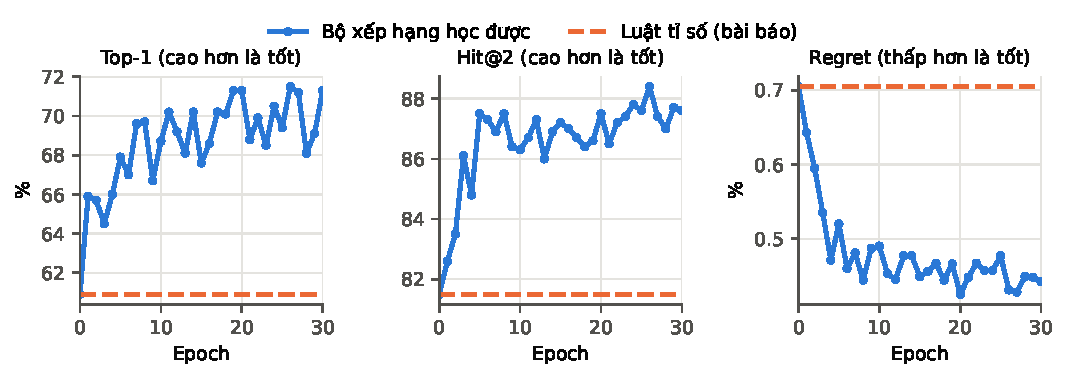
\includegraphics[width=\textwidth]{chapter4/image/ranker_training.pdf}
\caption[Chỉ số của bộ xếp hạng trên tập kiểm định qua các epoch]{Chỉ số trên tập kiểm định (10 instance chưa gặp) qua các epoch huấn luyện. Epoch 0 là mô hình chưa huấn luyện, trùng với luật tỉ số.}
\label{fig:ranker_training}
\end{figure}

\begin{table}[H]
\centering
\caption{Chất lượng xếp hạng trên tập kiểm định: luật tỉ số của E2LS so với bộ xếp hạng học được (checkpoint epoch 30).}
\label{tab:ranker_val}
\small
\begin{tabular}{lrrr}
\toprule
 & \textbf{Top-1 (\%)} & \textbf{Hit@2 (\%)} & \textbf{Regret (\%)}\\
\midrule
Luật tỉ số $R(S,i)$ & 60.9 & 81.5 & 0.705\\
Bộ xếp hạng học được & \textbf{71.3} & \textbf{87.6} & \textbf{0.442}\\
\bottomrule
\end{tabular}
\end{table}

Kết quả này cho thấy hai điều. Thứ nhất, luật tỉ số của E2LS đã khá tốt nhưng còn xa mức tối ưu: trong gần 40\% quyết định, ứng viên mà nó xếp đầu không phải là ứng viên tốt nhất, và trong 18.5\% quyết định, cả hai ứng viên được rẽ nhánh đều không tối ưu. Thứ hai, một mạng nơ-ron đồ thị nhỏ có thể học được phần lớn khoảng cách này từ dữ liệu: tỉ lệ chọn đúng tăng thêm 10.4 điểm phần trăm, tỉ lệ bỏ sót ứng viên tối ưu khỏi hai nhánh giảm từ 18.5\% xuống 12.4\%, và regret giảm 37\%. Vì tập kiểm định gồm các instance chưa gặp, mức cải thiện này phản ánh khả năng tổng quát hóa trong cùng phân phối kích thước ($m,n\le200$).

\section{Chi phí suy luận}\label{sec:cost}

Hàm xếp hạng học được phụ thuộc vào lời giải hiện tại nên phải được tính lại tại mỗi nút \addstar có nhiều hơn $a_{num}$ ứng viên. Để đo chi phí này, luận văn chạy 200 bước trên instance lớn nhất \texttt{sukp\_1000\_1000\_0.10\_0.75}, một lần với luật tỉ số và một lần với mạng (Bảng~\ref{tab:cost}).

\begin{table}[H]
\centering
\caption{Chi phí của 200 bước tìm kiếm trên \texttt{sukp\_1000\_1000\_0.10\_0.75} (CPU).}
\label{tab:cost}
\small
\begin{tabular}{lrr}
\toprule
 & \textbf{Luật tỉ số} & \textbf{Mạng}\\
\midrule
Thời gian cho 200 bước & 0.63 s & 4.03 s\\
Số lần gọi mạng & -- & 409\\
Thời gian một lần gọi mạng & -- & khoảng 9.5 ms\\
Thời gian trung bình mỗi nút \addstar (luật tỉ số) & khoảng 0.9 ms & --\\
\bottomrule
\end{tabular}
\end{table}

Mỗi lần gọi mạng tốn khoảng 9.5 mili giây, tức khoảng mười lần chi phí trung bình của một nút \addstar với luật tỉ số, và toàn bộ bước tìm kiếm chậm đi khoảng 6.4 lần. Chi phí này đến từ ba vòng truyền thông điệp trên ma trận kề dày kích thước $1000\times1000$ và từ việc gọi qua lại giữa C++ và Python. Hệ quả là ở cùng 30 giây, bộ giải dùng mạng chỉ thực hiện được khoảng một phần sáu số bước trên instance lớn. Vì vậy một hàm xếp hạng học được chỉ có lợi trong thực tế nếu chất lượng xếp hạng tốt hơn đủ để bù cho số bước bị mất. Điều này cần được kiểm chứng riêng ở chế độ cùng thời gian, và cũng là động lực cho các hướng giảm chi phí ở Chương~\ref{ch:chap5}.

\section{Đánh giá các hàm xếp hạng học được trên bộ chuẩn}\label{sec:pending}

Để đánh giá các hàm xếp hạng học được trên 60 instance chuẩn, luận văn đề xuất quy trình sau, được cài đặt trong \texttt{eval\_rankers.py} (Phụ lục~A). Mỗi cặp (instance, hàm xếp hạng) được chạy với ba seed trong hai chế độ ngân sách:
\begin{itemize}
  \item \textbf{Cùng số bước} (1000 bước tìm kiếm cục bộ): đo \emph{chất lượng xếp hạng}, vì hai bộ giải khám phá cùng số láng giềng và chỉ khác ở thứ tự rẽ nhánh của \addstar.
  \item \textbf{Cùng thời gian} (30 giây): đo \emph{giá trị thực tế}, vì thời gian suy luận của mạng được tính vào ngân sách.
\end{itemize}
Với DQN, chi phí huấn luyện trên từng instance phải được báo cáo cùng với thời gian giải. Kết quả được tổng hợp trong Bảng~\ref{tab:ranker_bench}; các ô đánh dấu đỏ sẽ được điền sau khi hoàn tất các lượt chạy.

\begin{table}[H]
\centering
\caption[Luật tỉ số so với các hàm xếp hạng học được trên bộ chuẩn]{Luật tỉ số so với các hàm xếp hạng học được trên bộ chuẩn (trung bình 3 seed). Gap: khoảng cách trung bình tới BKS. T/H/B: số instance thắng/hòa/thua so với luật tỉ số.}
\label{tab:ranker_bench}
\small
\begin{tabular}{llrrrr}
\toprule
\textbf{Ngân sách} & \textbf{Bộ} & \multicolumn{3}{c}{\textbf{Gap tới BKS (\%)}} & \textbf{T/H/B}\\
\cmidrule(lr){3-5}
 & & \textbf{Tỉ số} & \textbf{Xếp hạng} & \textbf{DQN} & \\
\midrule
1000 bước & Set I & \todo{...} & \todo{...} & \todo{...} & \todo{...}\\
1000 bước & Set II & \todo{...} & \todo{...} & \todo{...} & \todo{...}\\
30 giây & Set I & \todo{...} & \todo{...} & \todo{...} & \todo{...}\\
30 giây & Set II & \todo{...} & \todo{...} & \todo{...} & \todo{...}\\
\bottomrule
\end{tabular}
\end{table}

\section{Thảo luận}\label{sec:discussion}

\textbf{Bộ giải nền đủ mạnh để làm điểm so sánh.} Bản cài đặt C++ của E2LS với luật tỉ số đạt BKS trên 17/30 instance Set I chỉ trong 30 giây, không thua các thuật toán quần thể BABC và QL trên instance nào, và có khoảng cách trung bình 1.45\% trên Set II với ngân sách nhỏ hơn 33 lần so với E2LS gốc. Đây là một điểm so sánh chặt chẽ: một hàm xếp hạng học được phải cải thiện một bộ giải vốn đã mạnh, chứ không phải một bộ giải yếu.

\textbf{Luật tỉ số có dư địa cải thiện, và dư địa đó học được.} Trên các quyết định được gán nhãn chính xác, luật tỉ số chọn sai ứng viên tốt nhất ở gần 40\% số lần. Bộ xếp hạng học bắt chước giảm tỉ lệ này xuống còn khoảng 29\% trên instance chưa gặp, và giảm tỉ lệ bỏ sót ứng viên tối ưu khỏi hai nhánh của \addstar từ 18.5\% xuống 12.4\%. Nhờ cách tham số hóa dưới dạng hiệu chỉnh của luật tỉ số, mô hình bắt đầu từ đúng chất lượng của thuật toán gốc và chỉ thay đổi những chỗ có lợi.

\textbf{Câu hỏi còn mở là giá trị thực tế.} Có hai trở ngại giữa chất lượng xếp hạng tốt hơn và lời giải tốt hơn trên bộ chuẩn. Thứ nhất là \emph{tổng quát hóa theo kích thước}: bộ xếp hạng được huấn luyện trên $m,n\le200$ nhưng Set II có tới $m,n=1000$, và kinh nghiệm của DeepACO~\cite{Ye2023DeepACO} cho thấy mô hình học trên kích thước nhỏ vẫn có ích nhưng mất một phần lợi thế khi áp dụng cho kích thước lớn hơn nhiều. Thứ hai là \emph{chi phí suy luận}: ở cùng thời gian, bộ giải dùng mạng mất khoảng năm phần sáu số bước trên instance lớn (Mục~\ref{sec:cost}). Quy trình đánh giá ở Mục~\ref{sec:pending} được thiết kế để tách bạch hai yếu tố này: chế độ cùng số bước đo riêng chất lượng xếp hạng, còn chế độ cùng thời gian đo hiệu quả tổng thể.

\textbf{Khởi tạo lại là một điểm cắm tiềm năng khác.} Trên Set I, từ 21\% đến 44\% số bước kết thúc bằng khởi tạo lại, và thủ tục khởi tạo cũng dùng luật tỉ số. Một điểm số học được, tính một lần cho mỗi instance và dùng trong cả khởi tạo lẫn \addstar, có thể mang lại lợi ích mà gần như không tốn chi phí suy luận. Hướng này được thảo luận ở Chương~\ref{ch:chap5}.

\setcounter{figure}{0}
\setcounter{table}{0}
\mychapter{5}{Chương 5. Kết luận và hướng phát triển}\label{ch:chap5}

\section{Kết luận}

Luận văn nghiên cứu việc kết hợp tìm kiếm cục bộ với học máy cho bài toán cái túi hợp tập, theo nguyên tắc giữ nguyên một thuật toán mạnh và chỉ học lại đúng một thành phần của nó. Thành phần được chọn là bước xếp hạng ứng viên của toán tử \addstar trong E2LS, nơi bài báo gốc dùng tỉ số giá trị trên trọng số, một đánh giá tham lam một bước.

Các kết quả chính của luận văn như sau:
\begin{itemize}
  \item Luận văn cài đặt lại E2LS bằng C++ với trạng thái tăng dần, danh sách tabu bằng băm Zobrist và giao diện Python cho phép thay hàm xếp hạng. Với một lần chạy 30 giây, bộ giải đạt lời giải tốt nhất đã biết trên 17/30 instance của Set I, không thua các thuật toán quần thể BABC và QL trên instance nào, và có khoảng cách trung bình 1.45\% trên Set II dù ngân sách nhỏ hơn 33 lần so với công bố gốc.
  \item Luận văn mô hình hóa việc chọn nước đi thành một quá trình quyết định Markov với phần thưởng bằng mức cải thiện lời giải tốt nhất, và thiết kế một mạng nơ-ron đồ thị trên đồ thị hai phía item--element có số tham số không phụ thuộc kích thước instance. Mạng này được dùng chung cho hai phương án huấn luyện: DQN trên từng instance và bộ xếp hạng học bắt chước.
  \item Bộ xếp hạng học bắt chước, được tham số hóa như một hiệu chỉnh của luật tỉ số và huấn luyện từ nhãn tối ưu tính bằng tìm kiếm vét cạn, nâng tỉ lệ chọn đúng ứng viên tối ưu từ 60.9\% lên 71.3\%, nâng hit@2 từ 81.5\% lên 87.6\% và giảm regret 37\% trên các instance kiểm định chưa gặp. Toàn bộ quá trình huấn luyện mất dưới 10 phút trên CPU.
  \item Phân tích hành vi tìm kiếm cho thấy khởi tạo lại chiếm 21--44\% số bước trên các instance nhỏ, và việc gọi mạng tại mỗi nút \addstar làm bước tìm kiếm chậm đi khoảng 6.4 lần trên instance $1000\times1000$. Hai quan sát này xác định rõ những nơi mà học máy có thể đóng góp nhiều nhất với chi phí thấp nhất.
\end{itemize}

Nhìn chung, luận văn cho thấy luật xếp hạng viết tay của E2LS còn dư địa cải thiện đáng kể, và dư địa đó có thể học được bằng một mạng đồ thị nhỏ mà không cần thay đổi khung tìm kiếm. Việc chuyển chất lượng xếp hạng tốt hơn thành lời giải tốt hơn trên bộ chuẩn, khi đã tính cả chi phí suy luận, là bước tiếp theo của nghiên cứu.

\section{Hạn chế}

Luận văn còn một số hạn chế cần được ghi nhận rõ:
\begin{itemize}
  \item \textbf{Ngân sách thực nghiệm nhỏ.} Do chạy trên một máy tính xách tay, mỗi instance chỉ được chạy một lần trong 30 giây, trong khi các công bố dùng 500 đến 1000 giây và báo cáo kết quả tốt nhất của 10 lần chạy trở lên. Vì vậy luận văn không khẳng định được bộ giải đạt chất lượng ngang các công bố ở ngân sách chuẩn, và một lần chạy chưa cho biết độ biến động giữa các seed.
  \item \textbf{Bộ xếp hạng chưa được đánh giá trên bộ chuẩn.} Bộ xếp hạng học được mới được đánh giá về chất lượng xếp hạng trên các instance kiểm định sinh ngẫu nhiên; các lượt so sánh với luật tỉ số trên 60 instance chuẩn (Bảng~\ref{tab:ranker_bench}) chưa được hoàn tất.
  \item \textbf{Phương án DQN chưa được đánh giá đầy đủ.} Quy trình huấn luyện DQN đã được cài đặt và chạy thông, nhưng việc huấn luyện một mô hình cho mỗi trong 60 instance vượt quá khả năng tính toán của thực nghiệm này. Hơn nữa, vì DQN được huấn luyện trên chính instance cần giải, chi phí huấn luyện phải được tính vào thời gian giải nếu muốn so sánh công bằng với các thuật toán khác.
  \item \textbf{Nhãn chỉ có trên instance nhỏ.} Tìm kiếm vét cạn chỉ khả thi khi $m,n\le200$, nên bộ xếp hạng phải tổng quát hóa lên các instance lớn gấp năm lần kích thước huấn luyện.
  \item \textbf{Chi phí suy luận.} Mạng được gọi tại mỗi nút \addstar qua giao diện Python, với ma trận kề dày; chi phí này tăng nhanh theo kích thước instance và làm giảm số bước tìm kiếm trong cùng một khoảng thời gian.
\end{itemize}

\section{Hướng phát triển}

Từ các kết quả và hạn chế trên, luận văn đề xuất các hướng phát triển sau.

\textbf{Giảm chi phí suy luận.} Có thể chạy mạng trực tiếp trong C++ (chẳng hạn qua LibTorch), dùng ma trận kề thưa thay vì dày (mật độ của bộ chuẩn chỉ 10--15\%), và gom nhiều nút \addstar vào một lần gọi mạng. Một hướng triệt để hơn là tách mạng thành hai phần: phần nặng chỉ phụ thuộc instance được tính một lần, còn phần nhẹ phụ thuộc lời giải được tính tại mỗi nút.

\textbf{Điểm item học được tính một lần cho mỗi instance.} DeepACO~\cite{Ye2023DeepACO} cho thấy một heuristic học được, tính một lần cho mỗi instance rồi nhân vào heuristic chuyên gia, đã đủ để cải thiện rõ một metaheuristic mà gần như không tốn chi phí suy luận. Với SUKP, có thể dùng $\sigma(S,i)=\log R(S,i)+\beta\,h_\theta(i)$, trong đó $R(S,i)$ giữ phần phụ thuộc trạng thái và $h_\theta(i)$ là điểm của item do mạng tính một lần. Điểm này có thể dùng trong cả \addstar và thủ tục khởi tạo lại \textsc{Random\_Greedy}; trong thực nghiệm của luận văn, khởi tạo lại chiếm một phần đáng kể số bước tìm kiếm trên Set I.

\textbf{Huấn luyện bằng gradient chính sách.} Thay vì nhãn vét cạn, có thể huấn luyện bộ xếp hạng bằng REINFORCE như DeepACO: lấy mẫu nhiều cách hoàn thiện \addstar từ cùng một trạng thái, dùng lợi nhuận cuối làm phần thưởng và trung bình của các mẫu làm đường cơ sở. Cách này không cần nhãn nên huấn luyện được trực tiếp trên instance cỡ Set II, và có thể thưởng theo lợi nhuận \emph{sau vài bước tìm kiếm cục bộ} để mô hình học đúng điều mà bộ giải cần.

\textbf{Nhiễu loạn có hướng dẫn.} Khi mọi láng giềng đều tabu, thay vì khởi tạo lại từ đầu, có thể bỏ những item có điểm học được thấp nhất khỏi lời giải tốt nhất rồi điền lại bằng \addstar, để tìm kiếm tiếp tục ở gần vùng lời giải tốt.

\textbf{Đánh giá đầy đủ hơn.} Cần đánh giá với ngân sách chuẩn của các công bố (500 và 1000 giây, 10 lần chạy), huấn luyện và đánh giá DQN trên toàn bộ bộ chuẩn có tính chi phí huấn luyện, và mở rộng sang bộ Set III với tới 5000 item và sang bài toán BMCP mà E2LS cũng giải được.


\clearpage
\phantomsection
\addcontentsline{toc}{chapter}{Tài liệu tham khảo}
\bibliographystyle{plain}
\bibliography{reference}

\clearpage
\chapter*{Phụ lục A. Hướng dẫn tái lập kết quả}
\addcontentsline{toc}{chapter}{Phụ lục A. Hướng dẫn tái lập kết quả}
\setcounter{chapter}{0}
\renewcommand{\thesection}{A.\arabic{section}}
\setcounter{section}{0}
\sloppy

Toàn bộ mã nguồn, dữ liệu và kết quả của luận văn nằm trong kho mã \texttt{SUKP\_python}. Các lệnh dưới đây được chạy từ thư mục gốc của kho, trong môi trường ảo Python đã cài các gói trong \texttt{requirements.txt}.

\section{Biên dịch bộ giải C++}

\begin{lstlisting}[language=bash]
cmake -S . -B build -DPython_EXECUTABLE=$(which python)
cmake --build build -j
\end{lstlisting}
Lệnh này tạo module \texttt{sukp\_cpp} chứa bộ giải E2LS (thư mục \texttt{cpp\_solver/}).

\section{Huấn luyện bộ xếp hạng}

\begin{lstlisting}[language=bash]
python train_ranker.py --samples data/addback_samples.pt --epochs 30 \
    --out checkpoints/addback_ranker.pt
\end{lstlisting}
Lệnh này sinh 48 instance ngẫu nhiên, thu nhãn bằng tìm kiếm vét cạn, huấn luyện mạng và lưu checkpoint có hàm mất mát kiểm định nhỏ nhất. Nhật ký huấn luyện của luận văn được lưu tại \texttt{results\_csv/train\_ranker.log}.

\section{Huấn luyện DQN trên một instance}

\begin{lstlisting}[language=bash]
python train.py --config helper/config.yaml
\end{lstlisting}
Instance và siêu tham số được khai báo trong \texttt{helper/config.yaml}. Sổ tay \texttt{colab\_train.ipynb} chạy cùng các lệnh trên GPU của Google Colab cho toàn bộ bộ dữ liệu.

\section{Đánh giá trên 60 instance chuẩn}

\begin{lstlisting}[language=bash]
python eval_rankers.py --iterations 1000 --seeds 1 2 3 \
    --out results_csv/rankers_iter1000.csv
python eval_rankers.py --time 30 --seeds 1 2 3 \
    --out results_csv/rankers_time30.csv
python thesis/make_results.py
\end{lstlisting}
Hai lệnh đầu chạy bộ giải với luật tỉ số và với bộ xếp hạng học được, ở chế độ cùng số bước và cùng thời gian. Lệnh cuối sinh các bảng và hình của Chương~\ref{ch:chap4} từ các tệp CSV. Để chạy bộ giải trên instance khai báo trong \texttt{helper/config.yaml} với một hàm xếp hạng cụ thể, dùng \texttt{--ranker ratio} (luật tỉ số của bài báo), \texttt{--ranker network} (bộ xếp hạng học bắt chước) hoặc \texttt{--ranker dqn} (DQN đã huấn luyện cho instance đó):
\begin{lstlisting}[language=bash]
python play.py --ranker network --time 30
\end{lstlisting}


\end{document}
